% ============================================================================
%  Rapport de projet -- Projet 07
%  Communication sémantique apprise pour la transmission d'images et de vidéo
%
%  El Dabbabi Mouine · Saddoud Mohamed Amine · Bouchaala Oussema
%  Lakhader Mohamed Helmi            INSAT -- RT5 -- 2025/2026
%
%  Structure et charte reprises du rapport Genow (classe report, géométrie,
%  en-têtes, bibliographie ieeetr), adaptées à un projet académique.
%
%  Compilation :  pdflatex main && bibtex main && pdflatex main && pdflatex main
%          ou  :  latexmk -pdf main.tex
% ============================================================================
\documentclass[11pt,a4paper]{report}
% ============================================================================
%  Préambule partagé. Compatible pdfLaTeX (pas de fontspec), donc compilable
%  tel quel sur Overleaf, MiKTeX ou TeX Live.
%  Reprend la charte du rapport Genow : géométrie, couleurs, titres compacts,
%  en-têtes fancyhdr, listings, tableaux booktabs.
% ============================================================================
\usepackage[top=2.5cm, bottom=2.5cm, left=2.5cm, right=2.5cm, headheight=15pt]{geometry}
\usepackage[utf8]{inputenc}
\usepackage[T1]{fontenc}
\usepackage[french]{babel}
\usepackage{lmodern}
\usepackage{microtype}

\usepackage{graphicx}
\graphicspath{{figures/}}
\usepackage{setspace}
\usepackage{fancyhdr}
\usepackage{amsmath,amssymb,amsthm}
\usepackage{bm}
\usepackage{booktabs}
\usepackage{array}
\usepackage{tabularx}
\usepackage{longtable}
\usepackage{multirow}
\usepackage{makecell}
\usepackage{float}
\usepackage{caption}
\usepackage{subcaption}
\usepackage{upgreek}
\usepackage{siunitx}
\sisetup{detect-all, range-phrase=--, per-mode=symbol, output-decimal-marker={,}}
\DeclareSIPrefix{\micro}{\ensuremath{\upmu}}{-6}
\usepackage{textcomp}
\usepackage{pifont}
\usepackage[dvipsnames,table]{xcolor}
\usepackage{listings}
\usepackage{tikz}
\usetikzlibrary{arrows.meta,positioning,shapes.geometric,shapes.misc,fit,calc,backgrounds}
\usepackage[most]{tcolorbox}
\usepackage{enumitem}
\setlist{itemsep=2pt, topsep=4pt}
\usepackage{url}
\usepackage[hidelinks,bookmarksnumbered,hypertexnames=false]{hyperref}

\setstretch{1.2}
\setlength{\parskip}{0.3em}
\setlength{\emergencystretch}{3em}

% Titres de chapitre compacts : numéro et titre sur un seul bloc.
\usepackage{titlesec}
\titleformat{\chapter}[hang]{\normalfont\LARGE\bfseries\color{insatblue}}{\thechapter}{0.6em}{}[\vspace{2pt}\titlerule]
\titlespacing*{\chapter}{0pt}{-10pt}{14pt}
\titlespacing*{\section}{0pt}{10pt plus 2pt minus 2pt}{5pt plus 1pt}
\titlespacing*{\subsection}{0pt}{8pt plus 2pt minus 2pt}{3pt plus 1pt}
\captionsetup{font=small, labelfont=bf, skip=5pt}
\captionsetup[sub]{font=footnotesize}
\setlength{\textfloatsep}{12pt plus 2pt minus 3pt}
\setlength{\floatsep}{10pt plus 2pt minus 2pt}
\setlength{\intextsep}{10pt plus 2pt minus 2pt}

% Permet la coupure des identifiants monospace longs (power_normalize, ...).
\makeatletter
\let\tf@origtexttt\texttt
\renewcommand{\texttt}[1]{\tf@origtexttt{\tf@breakable{#1}}}
\newcommand{\tf@breakable}[1]{\begingroup\def\_{\textunderscore\allowbreak}#1\endgroup}
\makeatother

% ------------------------------------------------------------ éléments de base
\newcommand{\cmark}{\ding{51}}
\newcommand{\xmark}{\ding{55}}
\theoremstyle{definition}
\newtheorem{definition}{Définition}[chapter]

\pagestyle{fancy}
\fancyhf{}
\fancyhead[R]{\small\nouppercase\rightmark}
\fancyfoot[R]{\textbf{\thepage}}
\renewcommand{\headrulewidth}{0.4pt}
\fancypagestyle{plain}{\fancyhf{}\fancyfoot[R]{\textbf{\thepage}}\renewcommand{\headrulewidth}{0pt}}

% -------------------------------------------------------------------- couleurs
\definecolor{insatblue}{HTML}{1F4E9A}
\definecolor{codebg}{HTML}{F7F7F5}
\definecolor{codecomment}{HTML}{6A737D}
\definecolor{codekw}{HTML}{1F4E9A}
\definecolor{codestr}{HTML}{A33B00}
\definecolor{keyfill}{HTML}{EAF1FB}
\definecolor{keyframe}{HTML}{1F4E9A}
\definecolor{blk1}{HTML}{DCEAF9}
\definecolor{blk2}{HTML}{FDE5D8}
\definecolor{blk3}{HTML}{D7F2E7}
\definecolor{blk4}{HTML}{ECEAE4}

% -------------------------------------------------------------------- listings
\lstset{
  basicstyle=\ttfamily\footnotesize,
  backgroundcolor=\color{codebg},
  frame=single, rulecolor=\color{black!20},
  breaklines=true, breakatwhitespace=false,
  numbers=left, numberstyle=\tiny\color{codecomment}, numbersep=6pt,
  keywordstyle=\color{codekw}\bfseries,
  commentstyle=\color{codecomment}\itshape,
  stringstyle=\color{codestr},
  showstringspaces=false, tabsize=2, columns=fullflexible, keepspaces=true,
  captionpos=b, xleftmargin=1.5em, framexleftmargin=1.5em,
  literate={é}{{\'e}}1 {è}{{\`e}}1 {ê}{{\^e}}1 {à}{{\`a}}1 {ç}{{\c c}}1 {ù}{{\`u}}1
           {µ}{{$\mu$}}1 {°}{{\textdegree}}1 {→}{{$\rightarrow$}}1 {—}{{--}}1 {–}{{-}}1 {×}{{$\times$}}1
}
\renewcommand{\lstlistlistingname}{Liste des extraits de code}

% Encadré pour un résultat ou une idée clé.
\newtcolorbox{keybox}[1][]{colback=keyfill, colframe=keyframe, fonttitle=\bfseries\small,
  title={#1}, boxrule=0.6pt, arc=2pt, left=6pt, right=6pt, top=4pt, bottom=4pt, fontupper=\small}

% Référence à un fichier source du projet.
\newcommand{\srcfile}[1]{\texttt{\detokenize{#1}}}


\begin{document}

% ---------------------------------------------------------------- pages liminaires
\pagenumbering{roman}
% ----------------------------------------------------------------------------
%  Page de garde. Mise en page de l'en-tête institutionnel INSAT, adaptée à un
%  projet académique : ni entreprise, ni encadrant, ni page de validation.
% ----------------------------------------------------------------------------
\begin{titlepage}
\thispagestyle{empty}
\centering
\singlespacing

\begin{minipage}[c]{0.2\textwidth}
  
\includegraphics[width=2.8cm]{logo_insat.jpg}
\end{minipage}\hfill
\begin{minipage}[c]{0.56\textwidth}
  \centering\footnotesize
  \textsc{République Tunisienne}\\
  Ministère de l'Enseignement Supérieur et de la Recherche Scientifique\\[2pt]
  Université de Carthage\\[2pt]
  \textbf{Institut National des Sciences Appliquées et de Technologie}
\end{minipage}\hfill
\begin{minipage}[c]{0.2\textwidth}
  \raggedleft
\includegraphics[width=2.6cm]{logo_ucar.png}
\end{minipage}

\vspace{2pt}\rule{\textwidth}{0.6pt}

\vspace{0.9cm}
{\LARGE\textsc{Rapport de Projet}\par}
\vspace{0.5cm}
{\large Sciences Appliquées et Technologie\par}
\vspace{0.3cm}
{\large Spécialité : Réseaux Informatiques et Télécommunications\par}
{\large Niveau : 5\textsuperscript{e} année (RT5)\par}

\vspace{0.7cm}
\rule{0.85\textwidth}{0.8pt}\\[0.35cm]
{\Large\bfseries\color{insatblue}
Communication sémantique apprise pour la transmission d'images et de vidéo sur canal sans fil simulé\par}
\vspace{0.25cm}\rule{0.85\textwidth}{0.8pt}

\vspace{0.8cm}
{\large Réalisé par\par}
\vspace{0.35cm}
{\large\bfseries
\begin{tabular}{c@{\hspace{2.2cm}}c}
EL DABBABI Mouine & SADDOUD Mohamed Amine \\[0.35cm]
BOUCHAALA Oussema & LAKHADER Mohamed Helmi \\
\end{tabular}\par}

\vfill
\begin{tabular}{@{}r@{\hspace{0.6em}}l@{}}
  \textbf{Projet :} & Projet 07 -- Codage conjoint source-canal appris (deep JSCC)\\
  \textbf{Canaux étudiés :} & AWGN et Rayleigh par blocs, simulés\\
  \textbf{Jeux de données :} & CIFAR-10, Kodak, séquences vidéo CIF\\
\end{tabular}

\vspace{0.6cm}
{\large Année universitaire : \textbf{2025/2026}\par}
\end{titlepage}

% ----------------------------------------------------------------------------
%  Résumé / Abstract
% ----------------------------------------------------------------------------
\cleardoublepage
\phantomsection
\addcontentsline{toc}{chapter}{Résumé}
\markboth{Résumé}{Résumé}
\vspace*{1cm}
{\LARGE\bfseries\color{insatblue} Résumé\par}\vspace{2pt}\hrule\vspace{12pt}

\noindent
Ce projet compare trois manières de transmettre une image sur un canal sans fil bruité simulé, à budget
radio strictement identique. La première est la chaîne séparée de Shannon, telle qu'elle est déployée
aujourd'hui : codage de source, code convolutif, modulation QAM, décodage de Viterbi, le tout simulé bit
à bit. La deuxième est un codage conjoint source-canal profond (\emph{deep JSCC}) entraîné de bout en bout
sur une perte pixel. La troisième, proposée ici, reprend exactement la même architecture et ne modifie que
la fonction de perte : s'ajoutent à l'erreur quadratique un terme de caractéristiques et un terme de tâche
calculés à travers un classifieur gelé.

À architecture, bande et canal identiques, le système sémantique cède environ \SI{0.5}{\decibel} de PSNR
et gagne 10 à 14 points de précision chez un juge indépendant, en canal AWGN comme en canal de Rayleigh.
À \SI{0}{\decibel}, là où la chaîne séparée réelle tombe au niveau du hasard, les deux systèmes appris
restent exploitables : le codage conjoint supprime l'effet falaise. Deux extensions prolongent l'étude,
une transmission orientée tâche qui atteint une précision comparable avec 32 fois moins de bande, et un
renouvellement conditionnel des latents qui divise la bande par trois sur une scène vidéo statique. Les
limites sont énoncées explicitement : le canal est simulé, et sur de grandes images jamais vues à
l'entraînement la borne idéale de la chaîne séparée reste devant.

\vspace{10pt}
\noindent\textbf{Mots-clés :} communication sémantique, codage conjoint source-canal, apprentissage profond,
canal AWGN, évanouissement de Rayleigh, PSNR, SSIM, effet falaise, transmission orientée tâche.

\vspace{1.4cm}
{\LARGE\bfseries\color{insatblue} Abstract\par}\vspace{2pt}\hrule\vspace{12pt}

\noindent
This project compares three ways of sending an image over a simulated noisy wireless channel under a
strictly identical radio budget. The first is the separated Shannon chain as deployed today: source
coding, convolutional code, QAM modulation and Viterbi decoding, simulated bit by bit. The second is a
deep joint source-channel code (deep JSCC) trained end to end on a pixel loss. The third, proposed here,
keeps exactly the same architecture and changes only the loss function, adding a feature term and a task
term computed through a frozen classifier.

With identical architecture, bandwidth and channel, the semantic system gives up about \SI{0.5}{\decibel}
of PSNR and gains 10 to 14 accuracy points as measured by an independent judge, on AWGN as well as on
Rayleigh fading. At \SI{0}{\decibel}, where the real separated chain drops to chance level, both learned
systems remain usable: joint coding removes the cliff effect. Two extensions complete the study: a
task-oriented transmitter reaching comparable accuracy with 32 times less bandwidth, and conditional
replenishment of the latent tensor, which divides bandwidth by three on a static video scene. The
limitations are stated explicitly: the channel is simulated, and on large images never seen during
training the ideal bound of the separated chain remains ahead.

\vspace{10pt}
\noindent\textbf{Keywords:} semantic communication, joint source-channel coding, deep learning, AWGN
channel, Rayleigh fading, PSNR, SSIM, cliff effect, task-oriented transmission.


\tableofcontents
\listoffigures
\listoftables
\vspace{1.2cm}
\phantomsection
\addcontentsline{toc}{chapter}{Liste des abréviations}
{\LARGE\bfseries\color{insatblue} Liste des abréviations\par}\vspace{2pt}\hrule\vspace{10pt}

\begin{small}
\begin{tabular}{@{}p{1.6cm}p{5.3cm}@{\hspace{0.6cm}}p{1.6cm}p{5.3cm}@{}}
\toprule
AE & Auto-encodeur (\emph{auto-encoder}) & LLR & Log-rapport de vraisemblance \\
AWGN & Bruit blanc gaussien additif & MCS & Schéma de modulation et de codage \\
BER & Taux d'erreur binaire & MSE & Erreur quadratique moyenne \\
CE & Entropie croisée (\emph{cross-entropy}) & PSNR & Rapport signal sur bruit crête \\
CIF & \emph{Common Intermediate Format} (352$\times$288) & QAM & Modulation d'amplitude en quadrature \\
CNN & Réseau de neurones convolutif & QPSK & Modulation par déplacement de phase à 4 états \\
CR & Renouvellement conditionnel & ReLU & \emph{Rectified Linear Unit} \\
CSI & Information d'état du canal & RGB & Rouge-vert-bleu \\
DCT & Transformée en cosinus discrète & SNR & Rapport signal sur bruit \\
GOP & Groupe d'images (\emph{group of pictures}) & SSIM & Indice de similarité structurelle \\
JPEG & \emph{Joint Photographic Experts Group} & VGG & \emph{Visual Geometry Group} (architecture) \\
JSCC & Codage conjoint source-canal & ZF & Forçage à zéro (\emph{zero-forcing}) \\
\bottomrule
\end{tabular}
\end{small}

\vspace{14pt}
{\large\bfseries\color{insatblue} Principales notations\par}\vspace{8pt}

\begin{small}
\begin{tabular}{@{}p{2.2cm}p{12.6cm}@{}}
\toprule
$n$ & Nombre de valeurs réelles de l'image source, $n = 3HW$ \\
$k$ & Nombre de symboles complexes émis sur le canal \\
$k/n$ & Rapport de bande ; point de fonctionnement principal $1/12$ \\
$c$ & Nombre de canaux latents effectivement transmis ($k/n = c/96$) \\
$\sigma^2$ & Variance du bruit complexe, $\sigma^2 = 10^{-\mathrm{SNR}/10}$ \\
$h$ & Coefficient de canal de Rayleigh, $h \sim \mathcal{CN}(0,1)$ \\
$x,\ \hat{x}$ & Image émise et image reconstruite au récepteur \\
$z$ & Tenseur latent produit par l'encodeur \\
$\lambda_f,\ \lambda_t$ & Poids des termes de caractéristiques et de tâche dans la perte sémantique \\
\bottomrule
\end{tabular}
\end{small}


% ----------------------------------------------------------------- corps du rapport
\cleardoublepage
\pagenumbering{arabic}
% ============================================================================
%  INTRODUCTION GÉNÉRALE
% ============================================================================
\chapter*{Introduction générale}
\addcontentsline{toc}{chapter}{Introduction générale}
\markboth{Introduction générale}{Introduction générale}

Toute la théorie des communications construite depuis 1948 repose sur une idée de Shannon : transmettre, c'est
reproduire au récepteur, aussi exactement que possible, la suite de symboles choisie à l'émetteur, sans se
préoccuper de ce que ces symboles veulent dire~\cite{shannon1948}. Weaver distinguait pourtant déjà trois
niveaux de problème — le niveau technique (les symboles arrivent-ils ?), le niveau sémantique (le sens
arrive-t-il ?) et le niveau de l'efficacité (le destinataire agit-il correctement ?) — et constatait que seul le
premier avait été résolu~\cite{weaver1949}.

Ce découpage a produit l'architecture que nous utilisons tous les jours : on compresse la source d'un côté
(JPEG, H.264), on protège les bits de l'autre (code correcteur, modulation), et le théorème de séparation
garantit qu'aucune optimalité n'est perdue à les traiter séparément. La garantie est pourtant
\emph{asymptotique} : elle suppose des blocs infiniment longs et un canal dont on connaît la statistique.
Les images sont courtes, et le rapport signal sur bruit réel n'est jamais exactement celui qui a été prévu.

\paragraph{Problème.} Deux conséquences se manifestent. D'abord l'\textbf{effet falaise} : au-dessus du SNR de
conception la chaîne sature sans exploiter la marge disponible, et en dessous le décodeur décroche et l'image
est perdue d'un seul coup — pas dégradée, perdue. Ensuite le \textbf{mauvais critère} : la chaîne optimise la
fidélité pixel, alors que le destinataire est de plus en plus souvent une machine qui cherche seulement à
reconnaître le contenu. La question posée par ce projet est donc la suivante : \emph{à budget radio égal,
vaut-il mieux transmettre des pixels fidèles ou transmettre le sens ?}

\paragraph{Démarche et contributions.} Nous avons construit et mesuré trois systèmes complets dans des
conditions strictement identiques — même image, même rapport de bande, même canal, mêmes métriques. Le premier
est la chaîne séparée classique, simulée bit à bit et non approchée. Le deuxième est un codage conjoint
source-canal profond entraîné sur une perte pixel, qui reprend l'architecture de référence de la
littérature~\cite{bourtsoulatze2019}. Le troisième, notre proposition, est strictement le même réseau et ne
diffère que par la fonction de perte, à laquelle nous ajoutons un terme de caractéristiques et un terme de
tâche calculés à travers un classifieur gelé. Comme seule la perte change, tout écart de résultat lui est
imputable. Deux extensions complètent l'étude : une transmission orientée tâche et un renouvellement
conditionnel des latents en vidéo. L'ensemble est accompagné d'un simulateur interactif qui déroule une
transmission réelle étape par étape.

\paragraph{Organisation du rapport.} Le chapitre~\ref{chap:contexte} présente les fondements théoriques et
l'état de l'art. Le chapitre~\ref{chap:architecture} formule le problème, les exigences et l'architecture
retenue. Le chapitre~\ref{chap:separee} décrit le canal simulé et la chaîne séparée de référence. Le
chapitre~\ref{chap:jscc} détaille les systèmes appris et la perte sémantique. Le chapitre~\ref{chap:protocole}
expose le protocole d'évaluation et les métriques, en insistant sur l'indépendance des juges. Le
chapitre~\ref{chap:resultats} présente et analyse les résultats, y compris ceux qui nous sont défavorables. Le
chapitre~\ref{chap:extensions} traite les deux extensions, et le chapitre~\ref{chap:simulateur} l'outil
interactif développé pour explorer et vérifier la chaîne.

% ============================================================================
%  CHAPITRE 1 -- FONDEMENTS ET ÉTAT DE L'ART
% ============================================================================
\chapter{Fondements et état de l'art}
\label{chap:contexte}

Ce chapitre n'introduit que les notions utilisées par la suite : le théorème de séparation et ses limites, les
modèles de canal retenus, la chaîne numérique classique et ses mécanismes d'erreur, puis les travaux sur
lesquels s'appuie la communication sémantique apprise.

\section{Le théorème de séparation et sa limite pratique}
\label{sec:separation}

Shannon montre qu'un système de communication peut être décomposé sans perte d'optimalité en deux blocs
indépendants~\cite{shannon1948} : un \textbf{codage de source}, qui retire la redondance de l'information, et un
\textbf{codage de canal}, qui réintroduit une redondance calculée pour résister au bruit. C'est le fondement de
toutes les architectures déployées : JPEG puis Wi-Fi, H.264 puis 4G.

Ce résultat est cependant valable à la limite des blocs de longueur infinie, pour un canal stationnaire dont
la statistique est connue de l'émetteur. Trois hypothèses tombent en pratique :

\begin{itemize}
  \item \textbf{Les blocs sont courts.} Une image CIFAR-10 au point de fonctionnement étudié dispose de
        \num{256} symboles complexes, soit quelques centaines de bits utiles. Le gain asymptotique des codes
        correcteurs n'est pas atteint à cette longueur.
  \item \textbf{Le SNR réel diffère du SNR prévu.} L'émetteur choisit son schéma de modulation et de codage
        avant de connaître l'état exact du canal.
  \item \textbf{Le critère optimisé n'est pas celui du destinataire.} La chaîne minimise une distorsion de
        reconstruction, alors que la tâche finale est souvent une reconnaissance.
\end{itemize}

\begin{definition}[Effet falaise]
Comportement en tout-ou-rien d'une chaîne numérique conçue pour un SNR cible : au-dessus du seuil, la qualité
sature et la marge disponible n'est pas exploitée ; en dessous, le décodeur de canal décroche, le train binaire
devient faux et l'information source est perdue en bloc plutôt que dégradée progressivement.
\end{definition}

\section{Modèles de canal}
\label{sec:canaux}

Le rapport signal sur bruit s'exprime en décibels, $\mathrm{SNR_{dB}} = 10\log_{10}(P_{\text{signal}} /
P_{\text{bruit}})$. Une valeur de \SI{0}{\decibel} signifie autant de bruit que de signal, une valeur de
\SI{20}{\decibel} cent fois moins de bruit que de signal. Deux modèles sont utilisés dans ce travail.

\paragraph{Canal AWGN.} Le modèle thermique idéal : à chaque symbole complexe émis s'ajoute un bruit gaussien
indépendant,
\begin{equation}
  y = x + n, \qquad n \sim \mathcal{CN}(0,\sigma^2), \qquad \sigma^2 = 10^{-\mathrm{SNR_{dB}}/10} .
  \label{eq:awgn}
\end{equation}

\paragraph{Canal de Rayleigh par blocs.} Modèle d'une liaison mobile : le signal atteint le récepteur par
plusieurs trajets réfléchis dont les phases s'additionnent, de sorte que l'amplitude reçue devient aléatoire,
\begin{equation}
  y = h\,x + n, \qquad h \sim \mathcal{CN}(0,1) .
  \label{eq:rayleigh}
\end{equation}
Le coefficient $h$ est tiré une fois par image (d'où « par blocs ») et reste constant pendant toute sa
transmission. Le récepteur est supposé connaître $h$ (CSI parfaite) et divise par $h$ : cette
\textbf{égalisation par forçage à zéro} ramène le problème à un canal AWGN de rapport signal sur bruit
instantané $\mathrm{SNR}\cdot|h|^2$, où $|h|^2$ suit une loi exponentielle de moyenne 1. Lorsque le tirage est
défavorable, l'évanouissement est profond et toute l'image en souffre.

\paragraph{Contrainte de puissance.} Un émetteur ne peut pas augmenter librement son amplitude pour couvrir le
bruit. La puissance moyenne est donc normalisée à 1 par symbole complexe. Sans cette contrainte, un système
appris obtiendrait un gain trivial en amplifiant sa sortie, et la comparaison avec la chaîne numérique
perdrait tout sens.

\section{La chaîne numérique classique}
\label{sec:chaine_classique}

\paragraph{Modulation QAM.} Les bits sont groupés et associés aux points d'une constellation du plan complexe :
QPSK transporte 2~bits par symbole, la 16-QAM 4~bits, la 64-QAM 6~bits. Plus la constellation est dense, plus
le débit est élevé, mais plus les points sont proches et donc sensibles au bruit. Le \textbf{codage de Gray}
numérote les points de sorte qu'une confusion entre voisins immédiats ne coûte qu'un seul bit faux.

\paragraph{Code convolutif et poinçonnage.} Le code retenu est le code convolutif de contrainte $K=7$ et de
polynômes générateurs $(133,171)_8$, celui du Wi-Fi 802.11a~\cite{ieee80211a}. Chaque bit émis dépend des sept
derniers bits d'entrée. Le rendement natif $1/2$ est porté à $2/3$ ou $3/4$ par \textbf{poinçonnage}, c'est-à-dire
en supprimant certains bits de redondance selon un motif fixe.

\paragraph{Décodage souple et Viterbi.} Le démodulateur ne tranche pas entre 0 et 1 : pour chaque bit il calcule
un log-rapport de vraisemblance $\mathrm{LLR} = \log\big(P(0)/P(1)\big)$, dont le signe indique le bit le plus
probable et l'amplitude la confiance. L'algorithme de Viterbi~\cite{viterbi1967} recherche ensuite le chemin le
plus vraisemblable dans le treillis à $2^{K-1} = 64$ états. Tant que le canal reste au-dessus du seuil du code,
la correction est quasi parfaite ; en dessous, le décodeur choisit le mauvais chemin et les erreurs passent en
masse. Le couple (modulation, rendement) est appelé \textbf{MCS}.

\section{Travaux antérieurs}
\label{sec:etat_art}

\paragraph{Communication sémantique.} Le domaine a été reformulé récemment autour de l'idée de Weaver : ne
transmettre que ce qui modifie l'interprétation du destinataire~\cite{qin2021,gunduz2023}. Xie
\emph{et al.}~\cite{xie2021} ont proposé un système de bout en bout pour le texte, Zhang
\emph{et al.}~\cite{zhang2023} une variante dont l'émetteur ignore la tâche du récepteur, et Fu
\emph{et al.}~\cite{fu2023} une quantification vectorielle du latent.

\paragraph{JSCC profond pour l'image.} Bourtsoulatze \emph{et al.}~\cite{bourtsoulatze2019} ont introduit le
codage conjoint source-canal convolutif dont notre système syntaxique est la reprise : encodeur CNN, symboles
analogiques, canal inséré comme une couche du réseau, décodeur CNN. Kurka et Gündüz~\cite{kurka2021} ont montré
qu'un seul modèle peut couvrir plusieurs rapports de bande, propriété que nous exploitons par troncature des
canaux latents. Xu \emph{et al.}~\cite{xu2022} y ont ajouté des modules d'attention, Dai
\emph{et al.}~\cite{dai2022} une transformée non linéaire.

\paragraph{Vidéo et transmission orientée tâche.} DeepWiVe~\cite{tung2022} et la transmission sémantique
vidéo~\cite{wang2023} étendent l'approche aux séquences. Shao \emph{et al.}~\cite{shao2022} formulent la
transmission orientée tâche comme un goulot d'étranglement informationnel : ne transmettre que ce dont
l'inférence a besoin. Notre extension du chapitre~\ref{chap:extensions} en est une version simple et directe.

\paragraph{Pertes perceptuelles.} Le terme de caractéristiques de notre perte sémantique est une perte
perceptuelle au sens de Johnson \emph{et al.}~\cite{johnson2016} : comparer les activations internes d'un
réseau gelé plutôt que les pixels. La nouveauté n'est pas la perte elle-même, mais son usage dans une chaîne de
transmission et surtout le protocole de mesure qui l'accompagne (chapitre~\ref{chap:protocole}).

\begin{table}[H]
\centering
\caption{Positionnement des trois systèmes comparés dans ce projet}
\label{tab:positionnement}
\small
\begin{tabularx}{\textwidth}{@{}p{3.2cm}cc>{\raggedright\arraybackslash}X@{}}
\toprule
\textbf{Système} & \makecell{\textbf{Bits}\\\textbf{explicites}} & \makecell{\textbf{Effet}\\\textbf{falaise}} & \textbf{Critère optimisé} \\
\midrule
Chaîne séparée & \cmark & \cmark & distorsion de source, puis fiabilité binaire \\
JSCC syntaxique & \xmark & \xmark & erreur quadratique sur les pixels \\
JSCC sémantique & \xmark & \xmark & pixels \emph{et} caractéristiques \emph{et} tâche \\
\bottomrule
\end{tabularx}
\end{table}

% ============================================================================
%  CHAPITRE 2 -- PROBLÈME, EXIGENCES ET ARCHITECTURE
% ============================================================================
\chapter{Problème, exigences et architecture}
\label{chap:architecture}

\section{Formulation}
\label{sec:formulation}

Soit une image $x \in [0,1]^{3\times H\times W}$ et $n = 3HW$ le nombre de valeurs réelles à transmettre.
L'émetteur dispose de $k$ symboles complexes ; le récepteur produit une reconstruction $\hat{x}$ ou
directement une décision. Deux objectifs s'opposent : la \textbf{fidélité} ($\hat{x}$ ressemble à $x$ au sens
du pixel) et le \textbf{sens} ($\hat{x}$ conduit un système d'analyse indépendant à la même conclusion que
$x$). L'hypothèse du projet est qu'ils ne sont pas équivalents.

\section{Le budget radio}
\label{sec:budget}

Sans budget commun, il suffirait d'accorder plus de bande à un système pour le faire gagner. Le
\textbf{rapport de bande} est donc fixé :
\begin{equation}
  \frac{k}{n} = \frac{\text{symboles complexes émis}}{3HW \text{ valeurs réelles de la source}},
  \qquad \text{point principal : } \frac{k}{n} = \frac{1}{12}.
  \label{eq:kn}
\end{equation}

L'encodeur appris produit 16 canaux latents au stride 4 ; deux valeurs réelles formant un symbole complexe,
transmettre $c$ canaux donne
\begin{equation}
  \frac{k}{n} = \frac{c}{96}, \qquad c \in \{2,4,8,12,16\} \;\Longrightarrow\; \frac{k}{n} \in
  \left\{\tfrac{1}{48}, \tfrac{1}{24}, \tfrac{1}{12}, \tfrac{1}{8}, \tfrac{1}{6}\right\}.
  \label{eq:ratio_c}
\end{equation}

\begin{keybox}[Ce qui varie]
C'est $k$, jamais $n$ : le dénominateur est l'image elle-même. Changer le budget revient à couper des canaux
latents, l'image restant identique. Cette agilité suppose que $c$ soit tiré au hasard à l'entraînement, ce qui
ordonne les canaux par importance : un seul modèle couvre alors les cinq rapports~\cite{kurka2021}.
\end{keybox}

\section{Exigences}
\label{sec:exigences}

\begin{table}[H]
\centering
\caption{Exigences retenues pour que la comparaison soit recevable}
\label{tab:exigences}
\small
\begin{tabularx}{\textwidth}{@{}p{1.1cm}p{4.2cm}>{\raggedright\arraybackslash}X@{}}
\toprule
\textbf{Réf.} & \textbf{Exigence} & \textbf{Mise en œuvre} \\
\midrule
E1 & Budget radio identique & $k$ imposé aux trois chaînes par l'équation~\eqref{eq:kn} \\
E2 & Puissance normalisée à 1 & empêche le gain par amplification ; \srcfile{power_normalize()} \\
E3 & Même canal, mêmes tirages & AWGN et Rayleigh communs, graines fixées par point \\
E4 & Chaîne numérique exacte & chaque paquet codé, modulé, bruité, décodé par Viterbi \\
E5 & Juges indépendants & le classifieur de la perte n'est jamais celui de la mesure \\
E6 & Architecture identique & seule la perte distingue syntaxique et sémantique \\
E7 & Un seul modèle & SNR dans $[0,20]$~dB et bande tirés au hasard à l'entraînement \\
E8 & Reproductibilité & campagne relançable, résultats en CSV, figures régénérées par script \\
\bottomrule
\end{tabularx}
\end{table}

\section{Architecture d'ensemble}
\label{sec:archi}

\begin{figure}[H]
  \centering
  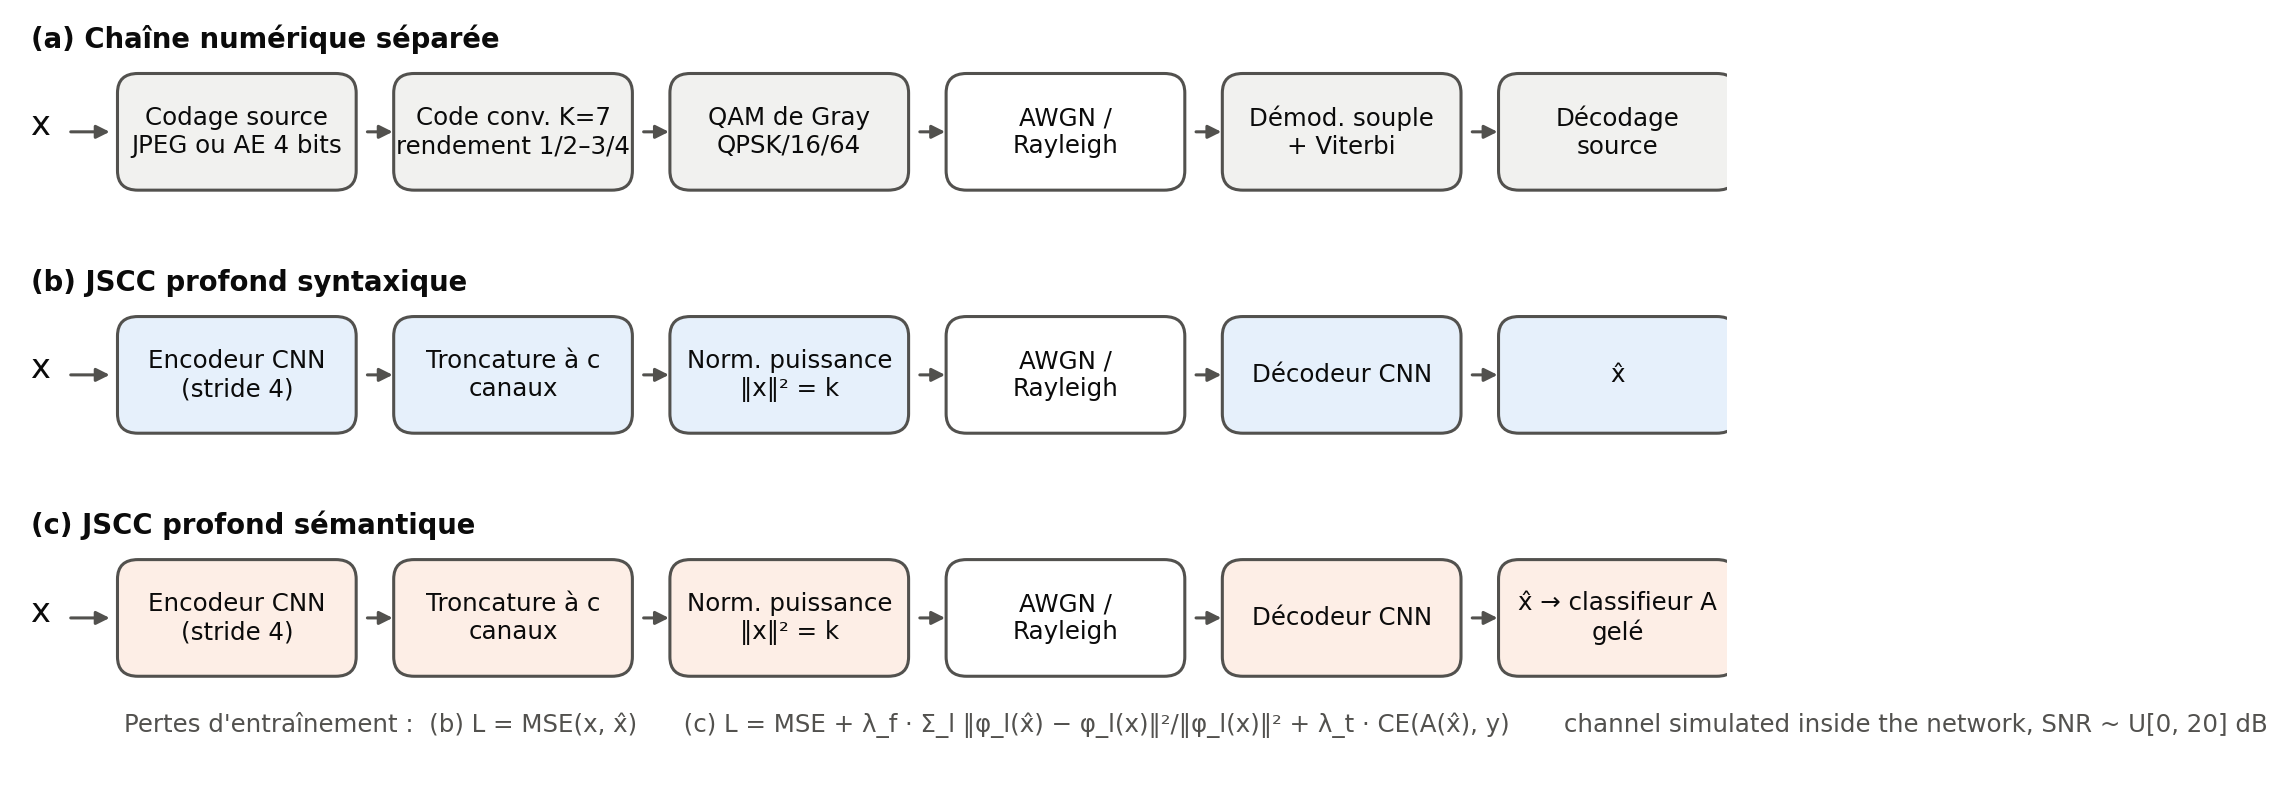
\includegraphics[width=\linewidth]{architecture.png}
  \caption{Les trois systèmes comparés : (a) chaîne numérique séparée, (b) JSCC syntaxique entraîné sur une
  perte pixel, (c) JSCC sémantique, de même architecture, entraîné avec les termes de caractéristiques et de
  tâche. Le canal simulé est commun aux trois.}
  \label{fig:architecture}
\end{figure}

\section{Organisation logicielle}
\label{sec:logiciel}

\begin{table}[H]
\centering
\caption{Organisation du code (Python et PyTorch)}
\label{tab:code}
\small
\begin{tabularx}{\textwidth}{@{}p{3.6cm}>{\raggedright\arraybackslash}X@{}}
\toprule
\textbf{Module} & \textbf{Contenu} \\
\midrule
\srcfile{semcom/channel.py} & normalisation de puissance, AWGN, Rayleigh avec égalisation ZF, troncature \\
\srcfile{semcom/models.py} & encodeur et décodeur JSCC, auto-encodeur 4 bits, classifieurs A et B, modèle de tâche \\
\srcfile{semcom/digital.py} & code convolutif, poinçonnage, QAM de Gray, LLR, Viterbi, débit JPEG \\
\srcfile{semcom/metrics.py} & PSNR, SSIM, métriques sémantiques ResNet-18 \\
\srcfile{semcom/data.py} & chargeurs CIFAR-10, Kodak et Y4M \\
\srcfile{semcom/train.py} & boucles d'entraînement, description des neuf modèles \\
\srcfile{semcom/video.py} & transmission image par image et renouvellement conditionnel \\
\srcfile{scripts/} & données, entraînement, évaluation, figures, démonstration, simulateur \\
\srcfile{explorer/} & simulateur interactif (chapitre~\ref{chap:simulateur}) \\
\bottomrule
\end{tabularx}
\end{table}

Tous les modèles d'image sont \textbf{entièrement convolutifs} : un réseau entraîné en $32\times32$
s'applique sans modification à des images $768\times512$ ou à des trames $352\times288$, pourvu que les
dimensions soient divisibles par 4. C'est ce qui rend possible l'évaluation par transfert du
chapitre~\ref{chap:resultats}.

% ============================================================================
%  CHAPITRE 3 -- CANAL SIMULÉ ET CHAÎNE SÉPARÉE
% ============================================================================
\chapter{Canal simulé et chaîne séparée}
\label{chap:separee}

La référence à battre doit être implémentée honnêtement, sinon la comparaison ne vaut rien.

\section{Le canal}
\label{sec:canal_impl}

Implémenté dans \srcfile{semcom/channel.py}, il enchaîne trois opérations communes aux trois systèmes.

\begin{enumerate}
  \item \textbf{Troncature} : seuls les $c$ premiers canaux latents sont émis, les autres sont mis à zéro au
        récepteur.
  \item \textbf{Normalisation} : la puissance moyenne vaut exactement 1 par symbole complexe,
        \begin{equation}
          x = z_{1:c}\sqrt{\frac{k}{\sum_i z_i^2}}, \qquad k = \tfrac{1}{2}\,\mathrm{card}(z_{1:c}) .
          \label{eq:power}
        \end{equation}
  \item \textbf{Bruit} : AWGN de variance $\sigma^2 = 10^{-\mathrm{SNR}/10}$, ou Rayleigh — tirage de
        $|h|^2$, SNR instantané $\mathrm{SNR}+10\log_{10}|h|^2$, puis même bruit.
\end{enumerate}

\section{Codage de source}
\label{sec:codage_source}

\paragraph{Grandes images : JPEG.} Sur Kodak et en vidéo, JPEG~\cite{wallace1992} à la plus haute qualité qui
tienne dans le budget. Au point $1/12$ en QPSK 1/2, une image Kodak dispose de \num{12216}~octets : la
qualité retenue est 6, pour \num{11084}~octets.

\paragraph{Petites images : auto-encodeur 4 bits.} Sur CIFAR-10, JPEG est inutilisable, et c'est mesuré. Le
tableau~\ref{tab:budget_cifar} donne le budget réel au point $1/12$ ($k = \num{256}$ symboles).

\begin{table}[H]
\centering
\caption{Budget utile par MCS pour une image CIFAR-10 à $k/n = 1/12$}
\label{tab:budget_cifar}
\small
\begin{tabular}{@{}lrrr@{}}
\toprule
\textbf{MCS} & \textbf{bits/symbole} & \textbf{bits utiles} & \textbf{octets} \\
\midrule
QPSK 1/2   & 1,0 & 248  & 31  \\
QPSK 3/4   & 1,5 & 376  & 47  \\
16-QAM 1/2 & 2,0 & 504  & 63  \\
16-QAM 3/4 & 3,0 & 760  & 95  \\
64-QAM 2/3 & 4,0 & 1016 & 127 \\
64-QAM 3/4 & 4,5 & 1136 & 142 \\
\bottomrule
\end{tabular}
\end{table}

Or le plus petit JPEG possible d'une image $32\times32$ pèse de \num{301} à \num{317}~octets : deux à dix fois
le budget. La cause est structurelle — marqueurs et tables de Huffman coûtent environ \num{300}~octets avant
le premier pixel, négligeables en $768\times512$ mais dominants en $32\times32$.

La chaîne emploie donc un auto-encodeur dont le latent est quantifié sur 4~bits (\srcfile{DigitalAE}),
entraîné sans canal : chaque canal latent coûte $64\times4 = \num{256}$~bits, soit 32~octets, et le budget de
142~octets en autorise 4. Ce choix \emph{avantage} délibérément la chaîne séparée.

\section{Codage de canal et réception}
\label{sec:canal_num}

Le train binaire est découpé en paquets d'au plus \num{1024}~bits utiles, terminés par 6~bits de queue. Chaque
paquet traverse : code convolutif $K=7$ poinçonné $\rightarrow$ QAM de Gray $\rightarrow$ canal $\rightarrow$
LLR max-log $\rightarrow$ Viterbi $\rightarrow$ décodage de source.

Rien n'est approché par une formule de taux d'erreur. Un fichier JPEG refusé par le décodeur devient une image
grise uniforme : le récepteur n'a rien d'autre à afficher.

\section{Trois formes de référence}
\label{sec:bornes}

\begin{description}[leftmargin=1.4cm, style=nextline]
  \item[MCS fixe] couple choisi d'avance : plafonne au-dessus du seuil, s'effondre en dessous.
  \item[Meilleur MCS] émetteur « génie » qui connaîtrait le SNR : meilleure adaptation de lien réalisable.
  \item[Borne de capacité] $k\log_2(1+\mathrm{SNR})$ bits \emph{sans erreur} : borne supérieure, pas un
        système constructible.
\end{description}

\begin{keybox}[Pourquoi encadrer la référence]
Battre une référence mal implémentée ne prouverait rien. En publiant les trois formes, on sait exactement ce
qui est dépassé : le chapitre~\ref{chap:resultats} montre que les systèmes appris dépassent largement la
chaîne réelle, dépassent la borne de capacité en précision sur CIFAR-10, mais restent en deçà de cette borne
en PSNR sur grandes images.
\end{keybox}

% ============================================================================
%  CHAPITRE 4 -- CODAGE CONJOINT SOURCE-CANAL APPRIS
% ============================================================================
\chapter{Codage conjoint source-canal appris}
\label{chap:jscc}

Ce chapitre décrit les deux systèmes appris : l'architecture commune, la manière dont le canal entre dans la
boucle d'apprentissage, puis la perte sémantique qui constitue la proposition du projet.

\section{Architecture}
\label{sec:archi_jscc}

Le principe du JSCC profond est de supprimer la frontière entre codage de source et codage de canal. Il n'y a
plus de bits : l'encodeur produit directement les symboles émis.

\paragraph{Encodeur.} Un réseau convolutif réduit l'image d'un facteur 4 en largeur et en hauteur
(deux convolutions de stride 2, suivies de deux blocs résiduels) et produit un tenseur latent
$z \in \mathbb{R}^{16 \times H/4 \times W/4}$. Les activations sont des PReLU.

\paragraph{Couche de canal.} Les valeurs latentes sont tronquées à $c$ canaux, normalisées en puissance, puis
bruitées selon le modèle choisi. Cette opération est \emph{différentiable} : le bruit traverse la
rétropropagation, de sorte que l'encodeur apprend un code adapté au canal plutôt qu'un code optimal en
l'absence de bruit.

\paragraph{Décodeur.} Un réseau symétrique — deux blocs résiduels puis deux convolutions transposées — remonte
à la résolution d'origine, avec une sigmoïde en sortie qui contraint l'image reconstruite dans $[0,1]$.

Le modèle complet compte \num{421715} paramètres. Les deux systèmes appris, syntaxique et sémantique,
partagent \emph{exactement} cette architecture ; leurs fichiers de poids ont la même taille et le même nombre
de paramètres. C'est l'exigence E6 du tableau~\ref{tab:exigences}.

\section{Protocole d'entraînement}
\label{sec:entrainement}

Tous les modèles sont entraînés sur les \num{50000} images d'apprentissage de CIFAR-10~\cite{krizhevsky2009},
avec augmentation par retournement horizontal et recadrage aléatoire, optimiseur Adam et pas d'apprentissage
$10^{-3}$.

Deux tirages aléatoires sont faits à chaque lot :

\begin{itemize}
  \item le \textbf{SNR}, uniformément dans $[0,20]$~dB, pour qu'un seul modèle couvre toute la plage
        d'exploitation ;
  \item le \textbf{nombre de canaux actifs} $c$ parmi $\{2,4,8,12,16\}$, pour l'agilité en bande.
\end{itemize}

Le tableau~\ref{tab:modeles} donne la liste des neuf modèles entraînés et leur coût.

\begin{table}[H]
\centering
\caption{Les neuf modèles entraînés (temps mesurés sur GPU)}
\label{tab:modeles}
\small
\begin{tabularx}{\textwidth}{@{}lrrr>{\raggedright\arraybackslash}X@{}}
\toprule
\textbf{Modèle} & \textbf{Époques} & \textbf{Paramètres} & \textbf{Durée (s)} & \textbf{Rôle} \\
\midrule
\srcfile{clsA}          & 10 & \num{298506} & \num{2296} & classifieur de la perte sémantique \\
\srcfile{clsB}          & 15 & \num{308394} & \num{3388} & juge indépendant \\
\srcfile{dae}           & 25 & \num{421715} & \num{7116} & codeur de source de la chaîne séparée \\
\srcfile{jscc_mse}      & 25 & \num{421715} & \num{8087} & JSCC syntaxique \\
\srcfile{jscc_sem}      & 25 & \num{421715} & \num{1346} & JSCC sémantique (proposition) \\
\srcfile{jscc_mse_snr0} & 15 & \num{421715} & \num{323}  & étude de désadaptation \\
\srcfile{jscc_mse_snr10}& 15 & \num{421715} & \num{349}  & étude de désadaptation \\
\srcfile{jscc_mse_snr20}& 15 & \num{421715} & \num{353}  & étude de désadaptation \\
\srcfile{task}          & 20 & \num{474266} & \num{370}  & extension orientée tâche \\
\bottomrule
\end{tabularx}
\end{table}

\begin{figure}[H]
  \centering
  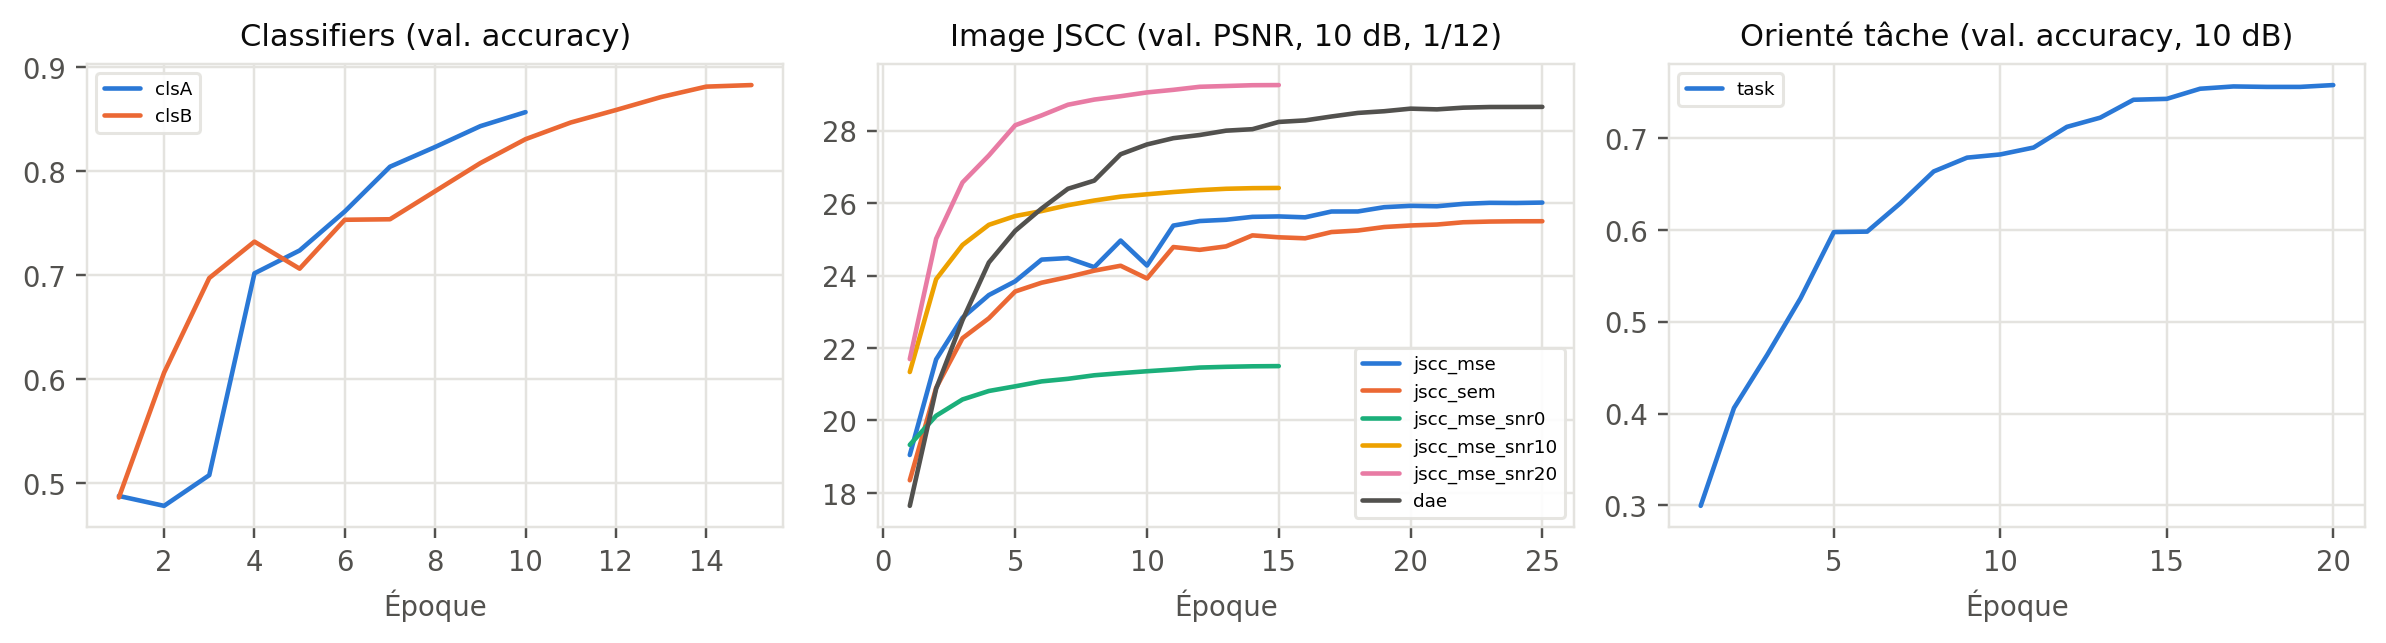
\includegraphics[width=0.78\linewidth]{learning_curves.png}
  \caption{Courbes d'apprentissage des principaux modèles : perte d'entraînement et métrique de validation.}
  \label{fig:learning}
\end{figure}

\section{Système syntaxique : la perte pixel}
\label{sec:jscc_mse}

Le premier système apprend à minimiser l'erreur quadratique moyenne entre l'image reçue et l'originale :
\begin{equation}
  \mathcal{L}_{\text{syn}} = \mathrm{MSE}(\hat{x}, x) .
  \label{eq:loss_mse}
\end{equation}
C'est la formulation de référence de la littérature~\cite{bourtsoulatze2019}. Elle demande des pixels justes,
et rien d'autre.

\section{Système sémantique : la proposition}
\label{sec:jscc_sem}

Le second système ne change \emph{que} la fonction de perte :
\begin{equation}
  \mathcal{L}_{\text{sem}} = \underbrace{\mathrm{MSE}(\hat{x},x)}_{\text{fidélité}}
  \;+\; \lambda_f \underbrace{\mathcal{L}_{\text{feat}}(\hat{x},x)}_{\text{caractéristiques}}
  \;+\; \lambda_t \underbrace{\mathrm{CE}\big(f_A(\hat{x}), y\big)}_{\text{tâche}},
  \qquad \lambda_f = 0{,}01,\; \lambda_t = 0{,}003 .
  \label{eq:loss_sem}
\end{equation}

\paragraph{Terme de caractéristiques.} Il compare les activations internes d'un classifieur $f_A$ \textbf{gelé}
pour l'image reçue et pour l'originale, normalisées par l'énergie de la carte de référence :
\begin{equation}
  \mathcal{L}_{\text{feat}}(\hat{x},x) = \frac{1}{L}\sum_{\ell=1}^{L}
  \frac{\mathrm{MSE}\big(f_A^{(\ell)}(\hat{x}),\, f_A^{(\ell)}(x)\big)}
       {\mathbb{E}\big[f_A^{(\ell)}(x)^2\big]} .
  \label{eq:loss_feat}
\end{equation}
C'est une perte perceptuelle au sens de Johnson \emph{et al.}~\cite{johnson2016} : elle demande que l'image
reste la même \emph{vue par un réseau}, et non pixel par pixel.

\paragraph{Terme de tâche.} L'entropie croisée entre la prédiction du classifieur gelé sur l'image reçue et
l'étiquette vraie. Il demande simplement que la classe reste décodable après transmission.

\paragraph{Pondération.} Les coefficients sont faibles — $1\%$ et $0{,}3\%$ — et ce choix est délibéré : le
sens est un \emph{ajout} à la fidélité, pas un remplacement. Une pondération plus forte produirait des images
flatteuses pour le classifieur mais visuellement dégradées, ce qui déplacerait le compromis au lieu de
l'améliorer.

\begin{keybox}[Pourquoi le classifieur est gelé]
$f_A$ n'est pas entraîné pendant l'optimisation du JSCC : ses poids sont figés et seuls les gradients le
traversent. S'il était entraîné conjointement, il lui suffirait de s'adapter aux artefacts du décodeur pour
faire baisser la perte sans que le sens soit mieux transmis. Le gel est donc une condition de validité, pas un
détail d'implémentation.
\end{keybox}

\section{Comparaison des signaux émis}
\label{sec:signaux}

La différence la plus visible entre les deux familles de systèmes apparaît dans le plan complexe. La chaîne
numérique émet des points discrets et réguliers — une constellation — et le bruit fait franchir des frontières
de décision, ce qui produit des bits faux. Le JSCC émet un \emph{nuage continu} : il n'y a pas de frontière à
franchir, donc pas de seuil, et le bruit se traduit par une dégradation graduelle de la reconstruction. C'est
l'explication directe de la disparition de l'effet falaise, que le chapitre~\ref{chap:resultats} quantifie et
que le simulateur du chapitre~\ref{chap:simulateur} donne à voir directement.

% ============================================================================
%  CHAPITRE 5 -- PROTOCOLE D'ÉVALUATION ET MÉTRIQUES
% ============================================================================
\chapter{Protocole d'évaluation et métriques}
\label{chap:protocole}

Mesurer « le sens » est le point délicat : un protocole mal construit produirait des chiffres flatteurs et
faux.

\section{Jeux de données}
\label{sec:donnees}

\begin{table}[H]
\centering
\caption{Jeux de données et rôle de chacun}
\label{tab:donnees}
\small
\begin{tabularx}{\textwidth}{@{}p{2.1cm}p{2.4cm}p{2.4cm}>{\raggedright\arraybackslash}X@{}}
\toprule
\textbf{Jeu} & \textbf{Taille} & \textbf{Usage} & \textbf{Remarque} \\
\midrule
CIFAR-10~\cite{krizhevsky2009} & $32\times32$, 10 classes & entraînement et évaluation & \num{50000} images d'apprentissage ; test sur les \num{5000} premières, pas de \SI{1}{\decibel} \\
Kodak~\cite{kodak} & $768\times512$, 24 images & évaluation seule & jamais vues à l'entraînement ; pas de \SI{2}{\decibel} \\
Vidéo CIF~\cite{xiph} & $352\times288$, 3 clips & évaluation seule & 30 premières trames d'\srcfile{akiyo} (statique), \srcfile{foreman} (modéré), \srcfile{bus} (rapide) \\
\bottomrule
\end{tabularx}
\end{table}

Les clips CIF remplacent les séquences UVG~\cite{uvg} suggérées initialement, dont les fichiers 1080p bruts
pèsent plusieurs gigaoctets. Les trois régimes de mouvement retenus s'avèrent déterminants pour l'extension
vidéo du chapitre~\ref{chap:extensions}.

\section{Métriques}
\label{sec:metriques}

\paragraph{Fidélité.} Le PSNR, en décibels,
\begin{equation}
  \mathrm{PSNR}(\hat{x},x) = 10\log_{10}\frac{1}{\mathrm{MSE}(\hat{x},x)} \quad \text{(images dans } [0,1]),
  \label{eq:psnr}
\end{equation}
vaut \SI{30}{\decibel} pour une bonne reconstruction et \SI{20}{\decibel} pour une image visiblement
dégradée. Le SSIM~\cite{wang2004}, entre 0 et 1, compare localement luminance, contraste et structure.

\paragraph{Sens.} Sur CIFAR-10, la \textbf{précision} d'un classifieur sur l'image reçue ; la référence sur
images originales est \textbf{88,4\,\%}. Sur Kodak et en vidéo, faute d'étiquette, un
ResNet-18~\cite{he2016} pré-entraîné sur ImageNet fournit la similarité cosinus des caractéristiques
(\srcfile{sem_cos}) et l'accord des étiquettes avant/après transmission (\srcfile{top1_agree}).

\section{L'indépendance des juges}
\label{sec:juges}

\begin{keybox}[Règle de séparation]
Le réseau qui intervient dans la perte n'est jamais celui qui mesure le résultat.
\end{keybox}

Sans cette séparation, le système sémantique pourrait apprendre à produire des artefacts qui plaisent à son
propre correcteur : la précision mesurée monterait sans que le sens soit mieux transmis.

\begin{table}[H]
\centering
\caption{Rôle de chaque réseau : apprentissage ou mesure, jamais les deux}
\label{tab:juges}
\small
\begin{tabularx}{\textwidth}{@{}p{3.4cm}ccX@{}}
\toprule
\textbf{Réseau} & \makecell{\textbf{Dans une}\\\textbf{perte}} & \makecell{\textbf{Utilisé pour}\\\textbf{mesurer}} & \textbf{Précision sur images originales} \\
\midrule
Classifieur A (ResNet) & \cmark & \xmark & 85,4\,\% \\
Classifieur B (VGG) & \xmark & \cmark & 88,4\,\% \\
ResNet-18 ImageNet & \xmark & \cmark & référence de similarité sémantique \\
\bottomrule
\end{tabularx}
\end{table}

\section{Conduite des mesures}
\label{sec:mesures}

Pour chaque couple (MCS, SNR), les paquets de toutes les images sont codés, modulés, envoyés et décodés par
Viterbi. Les graines sont fixées par point de mesure. Chaque scheme produit une ligne de CSV dans
\srcfile{results/eval/} ; tableaux et figures en sont dérivés par \srcfile{scripts/make_figures.py}, sans
recopie manuelle.

% ============================================================================
%  CHAPITRE 6 -- RÉSULTATS ET ANALYSE
% ============================================================================
\chapter{Résultats et analyse}
\label{chap:resultats}

Tous les chiffres proviennent de \srcfile{results/eval/}. Sauf mention contraire : $k/n = 1/12$, canal AWGN.

\section{CIFAR-10 : le résultat central}
\label{sec:res_cifar}

\begin{table}[H]
\centering
\caption{CIFAR-10, $k/n = 1/12$, AWGN. Référence : 88,4\,\% sur images originales.}
\label{tab:cifar}
\small
\begin{tabular}{@{}llrrr@{}}
\toprule
\textbf{SNR} & \textbf{Système} & \textbf{PSNR (dB)} & \textbf{SSIM} & \textbf{Précision} \\
\midrule
\multirow{4}{*}{\SI{0}{\decibel}}
 & JSCC syntaxique            & 20,08 & 0,669 & 42,0\,\% \\
 & \textbf{JSCC sémantique}   & \textbf{19,68} & \textbf{0,677} & \textbf{56,4\,\%} \\
 & Séparé — borne de capacité & 19,65 & 0,600 & 15,3\,\% \\
 & Séparé — meilleur MCS      & 12,63 & 0,132 & 9,8\,\% \\
\midrule
\multirow{4}{*}{\SI{10}{\decibel}}
 & JSCC syntaxique            & 25,99 & 0,874 & 67,6\,\% \\
 & \textbf{JSCC sémantique}   & \textbf{25,48} & \textbf{0,874} & \textbf{78,2\,\%} \\
 & Séparé — borne de capacité & 24,51 & 0,808 & 29,7\,\% \\
 & Séparé — meilleur MCS      & 19,65 & 0,600 & 15,3\,\% \\
\midrule
\multirow{4}{*}{\SI{20}{\decibel}}
 & JSCC syntaxique            & 27,72 & 0,906 & 70,6\,\% \\
 & \textbf{JSCC sémantique}   & \textbf{27,15} & \textbf{0,903} & \textbf{80,2\,\%} \\
 & Séparé — borne de capacité & 27,33 & 0,896 & 67,4\,\% \\
 & Séparé — meilleur MCS      & 25,71 & 0,850 & 40,5\,\% \\
\bottomrule
\end{tabular}
\end{table}

\begin{enumerate}
  \item \textbf{Le compromis sémantique est constant} : $\approx$\SI{0.5}{\decibel} de PSNR cédé, 10 à
        14~points de précision gagnés, à tous les SNR, sans dégradation du SSIM. Les pixels sacrifiés
        n'étaient pas ceux qui portaient le sens.
  \item \textbf{L'effet falaise est massif} : à \SI{0}{\decibel}, la chaîne séparée réelle donne 9,8\,\%, le
        niveau du hasard sur dix classes, contre 42\,\% et 56,4\,\% pour les systèmes appris.
  \item \textbf{La borne idéale est dépassée en précision} : elle ne corrige pas le \emph{critère}, son
        codeur de source optimisant toujours la fidélité pixel.
\end{enumerate}

\begin{figure}[H]
  \centering
  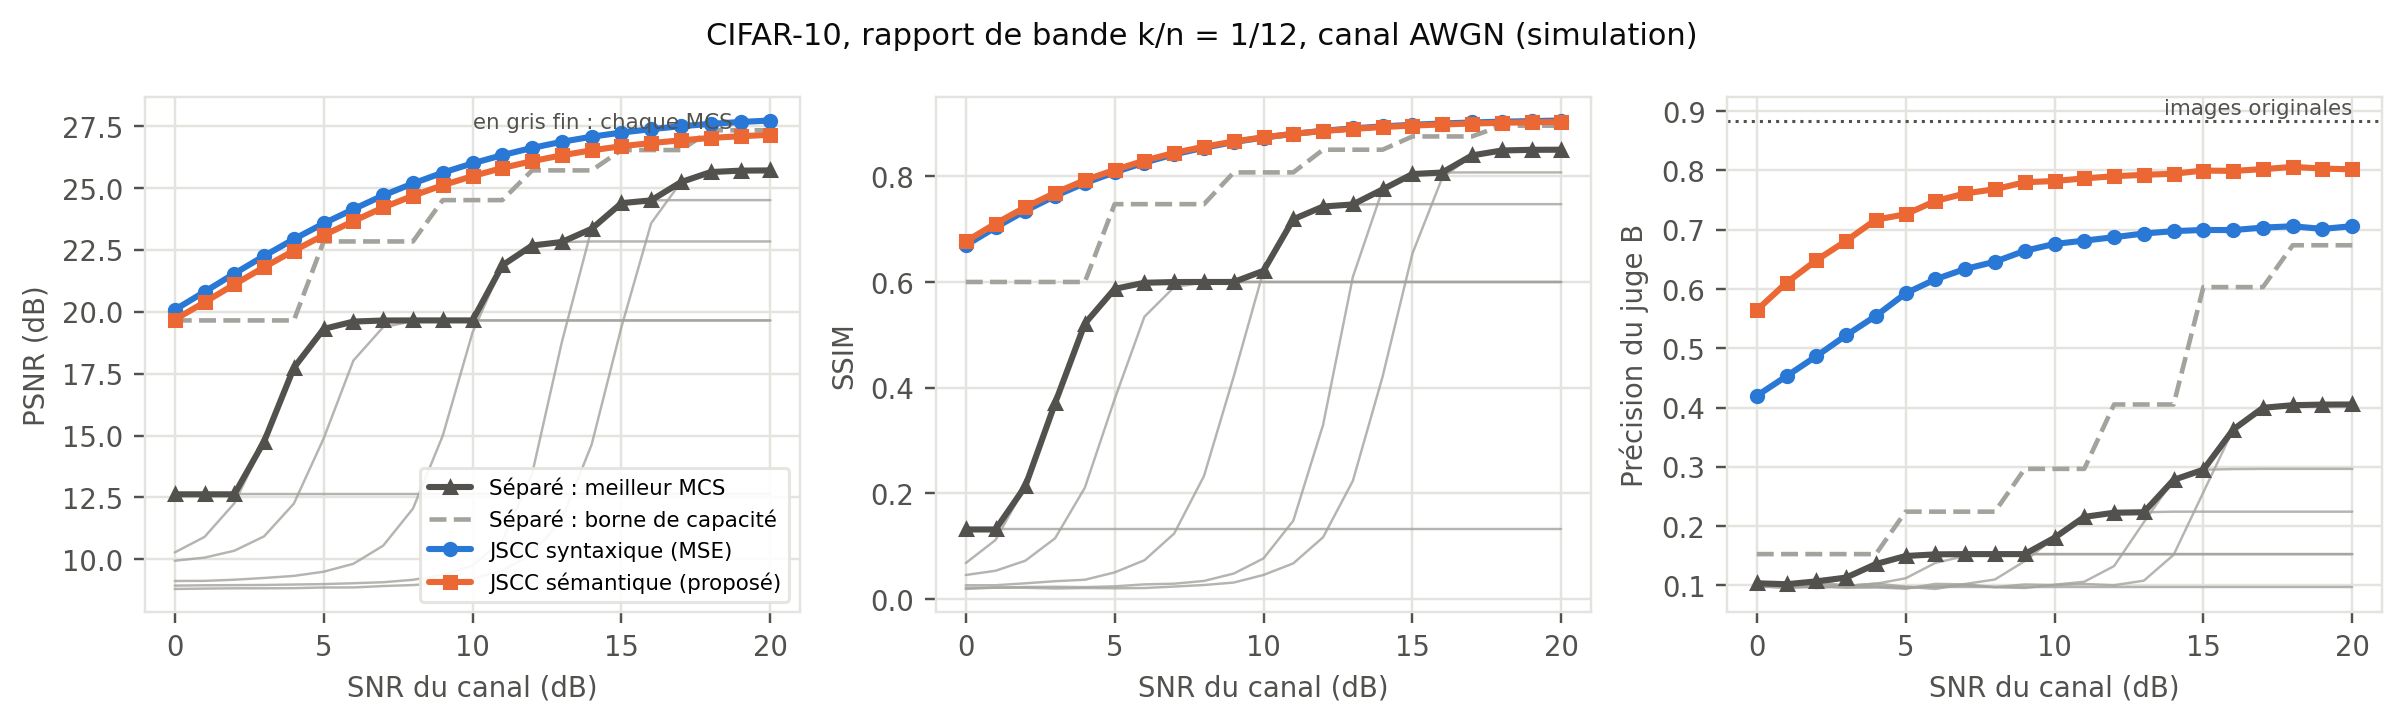
\includegraphics[width=0.80\linewidth]{cifar_snr.png}
  \caption{CIFAR-10 à $k/n = 1/12$ en fonction du SNR. Les courbes fines sont les MCS fixes de la chaîne
  séparée : leur plafonnement puis leur effondrement est l'effet falaise.}
  \label{fig:cifar_snr}
\end{figure}

\section{Influence du rapport de bande}
\label{sec:res_bande}

\begin{figure}[H]
  \centering
  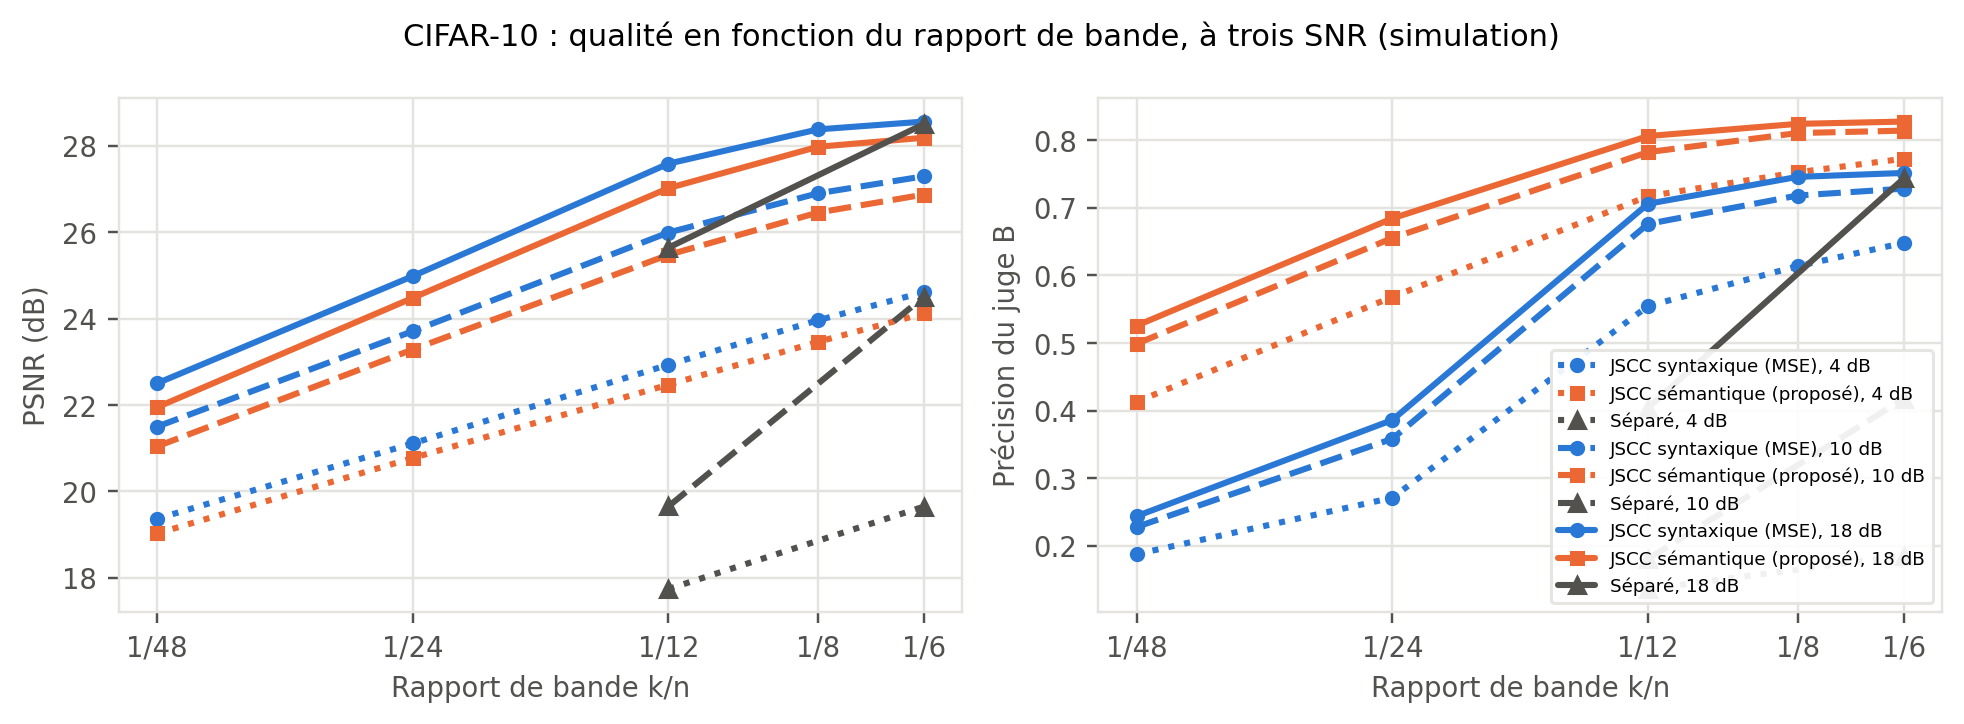
\includegraphics[width=0.96\linewidth]{cifar_bandwidth.png}
  \caption{Compromis débit/qualité sur CIFAR-10 à trois SNR. Un seul modèle couvre les cinq rapports $k/n$ ;
  les points noirs sont la chaîne séparée au meilleur MCS.}
  \label{fig:cifar_bandwidth}
\end{figure}

La chaîne séparée n'apparaît qu'aux deux budgets les plus larges : en dessous, le budget de bits ne permet
même pas un canal latent complet. À \SI{4}{\decibel} et $k/n = 1/12$, le meilleur MCS ne fait passer
qu'\emph{un seul} canal sur seize, le reste partant en redondance et en modulation prudente.

\section{Canal de Rayleigh}
\label{sec:res_rayleigh}

\begin{table}[H]
\centering
\caption{CIFAR-10 sur Rayleigh par blocs, \SI{10}{\decibel}, $k/n = 1/12$}
\label{tab:rayleigh}
\small
\begin{tabular}{@{}lrr@{}}
\toprule
\textbf{Système} & \textbf{PSNR (dB)} & \textbf{Précision} \\
\midrule
JSCC syntaxique          & 24,32 & 60,3\,\% \\
\textbf{JSCC sémantique} & 23,84 & \textbf{72,4\,\%} \\
\bottomrule
\end{tabular}
\end{table}

Même compromis qu'en AWGN — \SI{0.5}{\decibel} cédé, 12~points gagnés : le bénéfice ne dépend pas du modèle
de canal.

\begin{figure}[H]
  \centering
  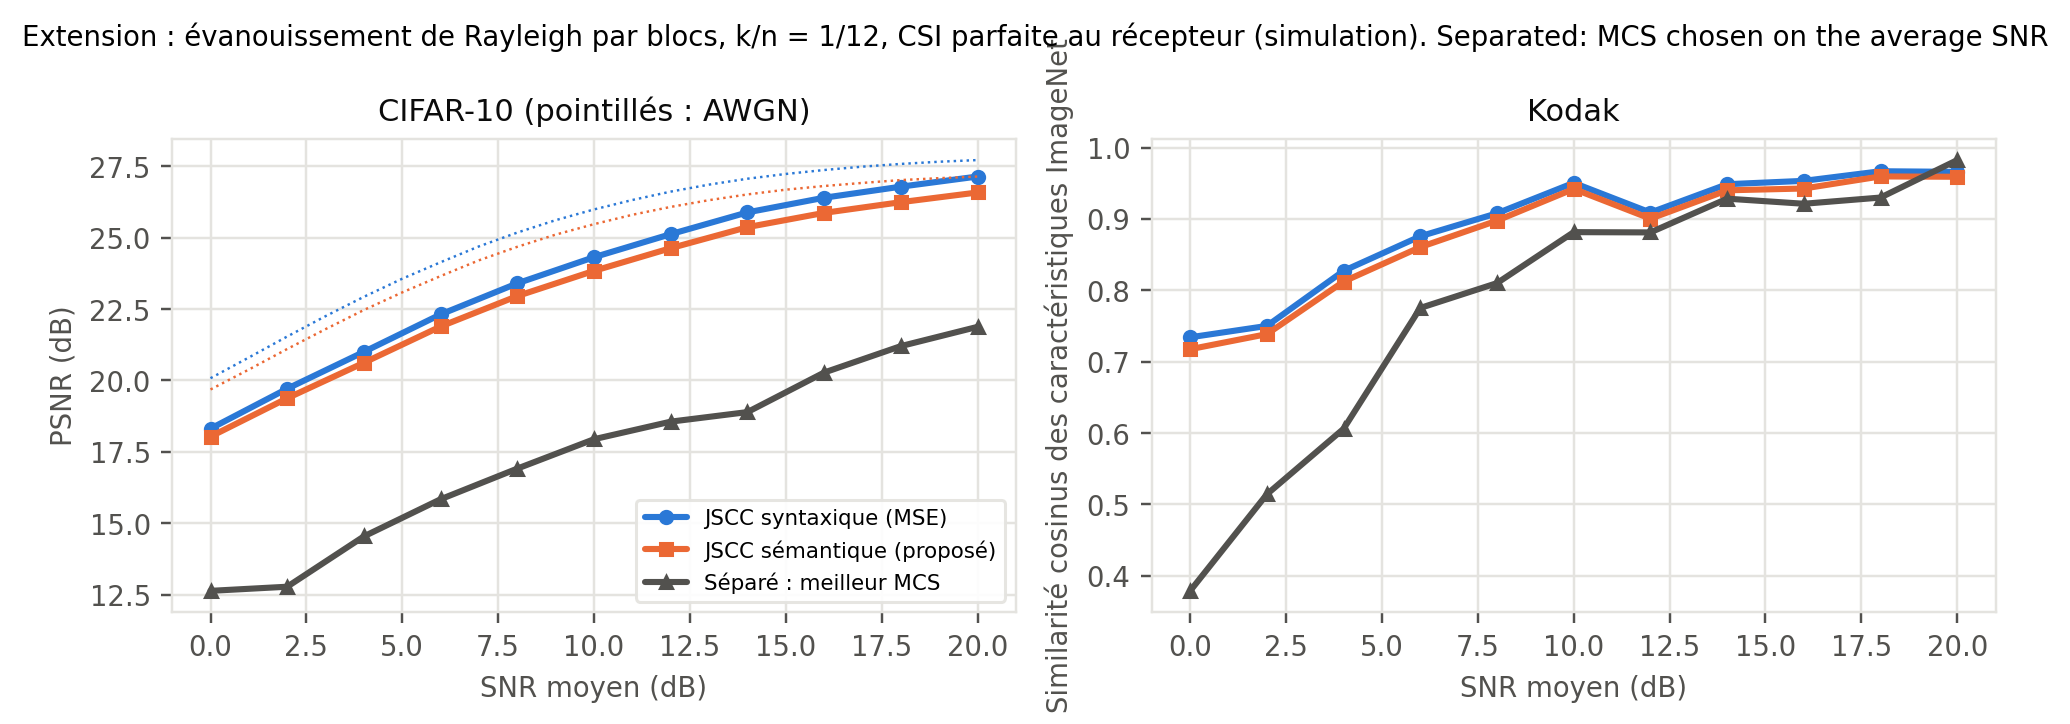
\includegraphics[width=0.94\linewidth]{rayleigh.png}
  \caption{Évanouissement de Rayleigh par blocs, CSI parfaite et égalisation par forçage à zéro.}
  \label{fig:rayleigh}
\end{figure}

\section{Désadaptation train/test du SNR}
\label{sec:res_mismatch}

\begin{table}[H]
\centering
\caption{Précision du juge B pour trois modèles entraînés à SNR fixe, $k/n = 1/12$}
\label{tab:mismatch}
\small
\begin{tabular}{@{}lrrr@{}}
\toprule
\textbf{Entraîné à} & \textbf{testé \SI{0}{\decibel}} & \textbf{testé \SI{10}{\decibel}} & \textbf{testé \SI{20}{\decibel}} \\
\midrule
\SI{0}{\decibel}  & 28,9\,\% & 30,2\,\% & 30,5\,\% \\
\SI{10}{\decibel} & 39,6\,\% & 69,5\,\% & 73,7\,\% \\
\SI{20}{\decibel} & 33,9\,\% & 67,3\,\% & 75,1\,\% \\
\bottomrule
\end{tabular}
\end{table}

Le modèle entraîné à \SI{0}{\decibel} plafonne à 30\,\% même en excellentes conditions : il n'exploite plus
la marge. Celui entraîné à \SI{20}{\decibel} s'effondre dès que le canal se dégrade. D'où la règle :
\textbf{entraîner sur une plage de SNR, jamais à un point fixe}.

\begin{figure}[H]
  \centering
  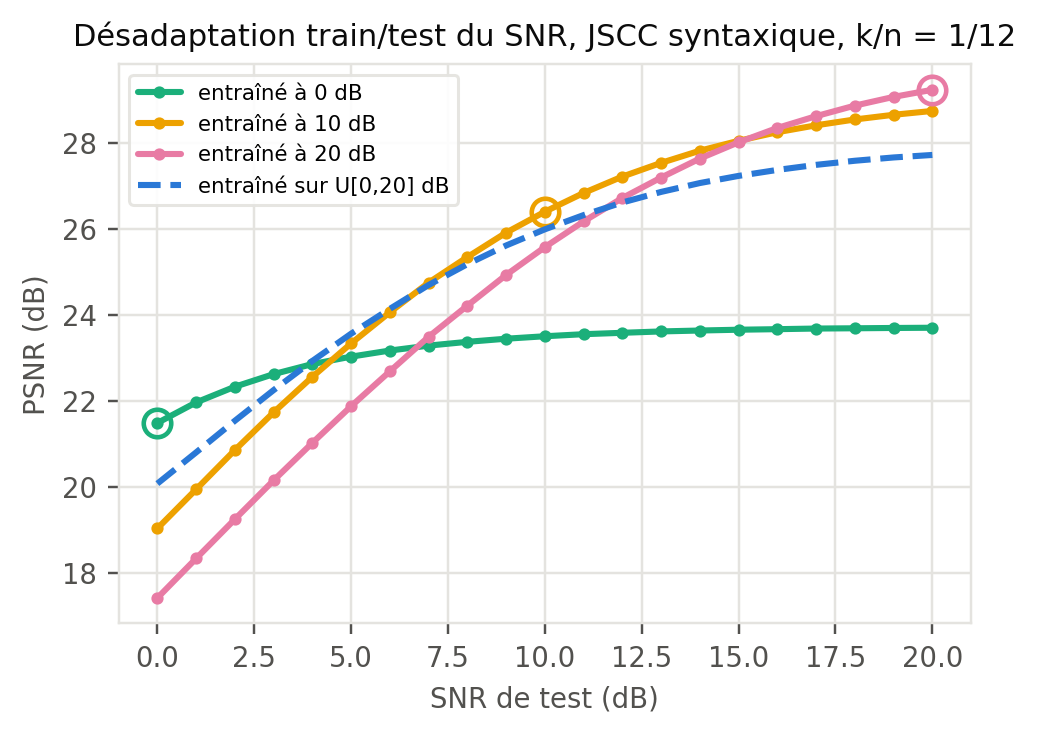
\includegraphics[width=0.88\linewidth]{snr_mismatch.png}
  \caption{Désadaptation train/test. Le cercle marque le point de conception ; la courbe en tirets est le
  modèle entraîné sur la plage complète.}
  \label{fig:mismatch}
\end{figure}

\section{Kodak et vidéo : le résultat défavorable}
\label{sec:res_kodak}

\begin{table}[H]
\centering
\caption{PSNR (dB) sur Kodak et vidéo, $k/n = 1/12$, AWGN}
\label{tab:kodak}
\small
\begin{tabular}{@{}llrrrr@{}}
\toprule
\textbf{Jeu} & \textbf{SNR} & \textbf{JSCC synt.} & \textbf{JSCC sém.} & \textbf{Séparé (capacité)} & \textbf{Séparé (meilleur MCS)} \\
\midrule
Kodak & \SI{0}{\decibel}  & 22,97 & 22,73 & \textbf{26,70} & 12,82 \\
Kodak & \SI{10}{\decibel} & 27,11 & 27,34 & \textbf{32,27} & 29,77 \\
Vidéo & \SI{0}{\decibel}  & 21,93 & 21,77 & \textbf{25,28} & 10,41 \\
Vidéo & \SI{10}{\decibel} & 26,59 & 26,62 & \textbf{31,95} & 29,11 \\
\bottomrule
\end{tabular}
\end{table}

Sur les grandes images, la borne de capacité l'emporte. Deux raisons, qu'il faut énoncer sans les atténuer :
les modèles n'ont été entraînés qu'en $32\times32$ et sont ici appliqués par transfert, terrain où JPEG est
chez lui ; et cette borne suppose zéro erreur, donc n'est pas réalisable.

Face au \emph{vrai} système séparé, la hiérarchie s'inverse dans les mauvaises conditions : à
\SI{0}{\decibel} sur Kodak, \SI{12.82}{\decibel} et 0\,\% d'accord top-1 contre $\approx$\SI{23}{\decibel}
pour les JSCC.

\begin{figure}[H]
  \centering
  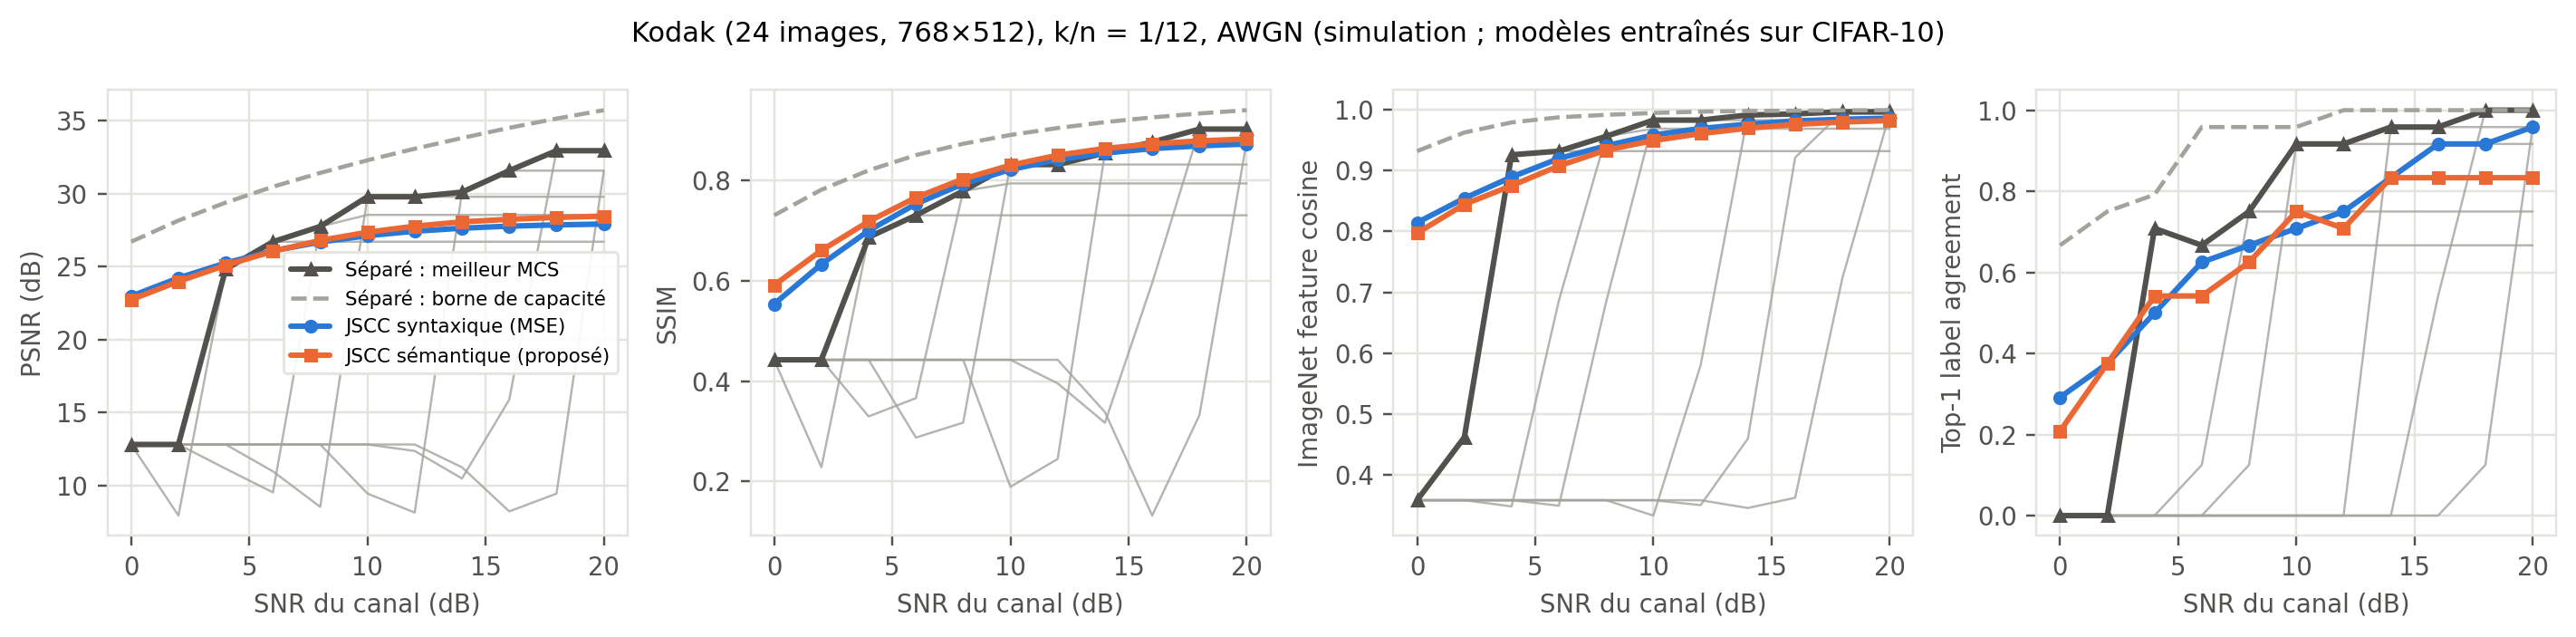
\includegraphics[width=0.76\linewidth]{kodak_snr.png}
  \caption{Kodak, 24 images $768\times512$ jamais vues à l'entraînement.}
  \label{fig:kodak}
\end{figure}

\begin{figure}[H]
  \centering
  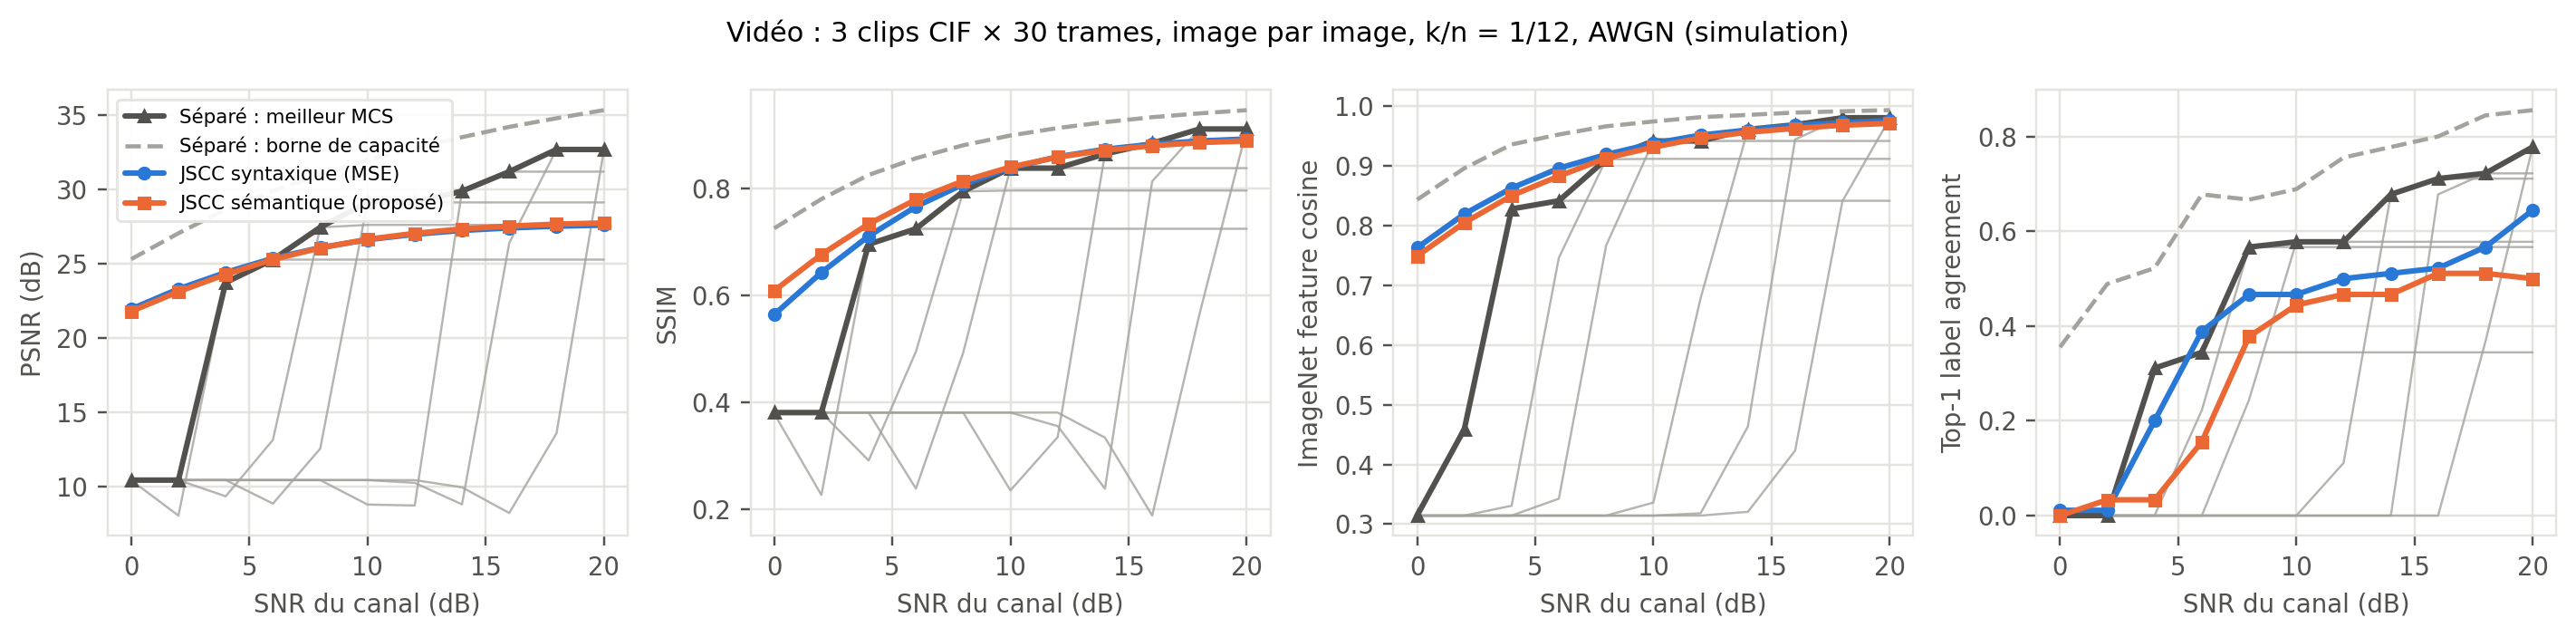
\includegraphics[width=0.76\linewidth]{video_snr.png}
  \caption{Vidéo : trois clips CIF, transmission image par image.}
  \label{fig:video}
\end{figure}

\begin{figure}[H]
  \centering
  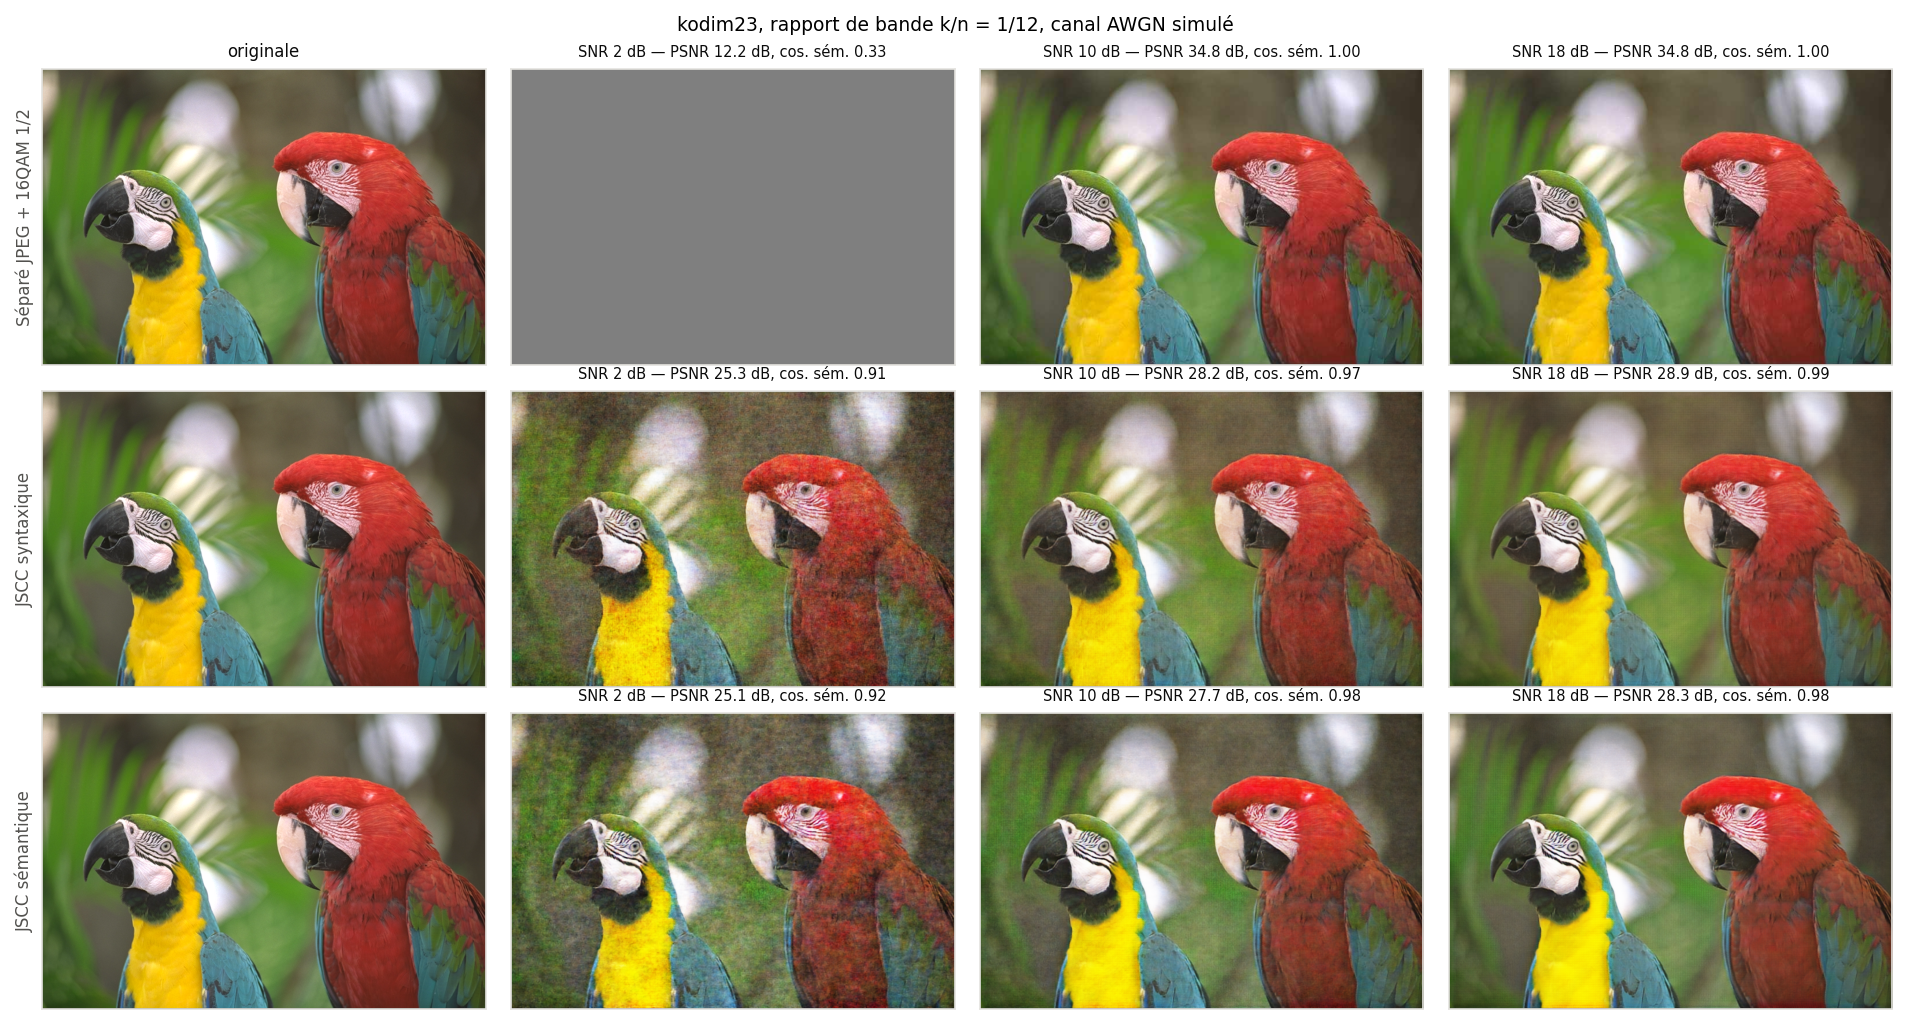
\includegraphics[width=\linewidth]{visual.png}
  \caption{Même image Kodak transmise par les trois systèmes, à trois SNR, au même budget.}
  \label{fig:visual}
\end{figure}

\section{Synthèse}
\label{sec:res_synthese}

\begin{keybox}[Ce que les mesures établissent]
\begin{enumerate}[leftmargin=1.2em]
  \item Le terme sémantique échange $\approx$\SI{0.5}{\decibel} de PSNR contre 10 à 14~points de précision,
        en AWGN comme en Rayleigh.
  \item Le codage conjoint supprime l'effet falaise.
  \item Entraîner sur une plage de SNR est indispensable.
  \item Sur grandes images non vues à l'entraînement, la borne séparée idéale reste devant en PSNR.
\end{enumerate}
\end{keybox}

% ============================================================================
%  CHAPITRE 7 -- EXTENSIONS
% ============================================================================
\chapter{Extensions}
\label{chap:extensions}

\section{Transmission orientée tâche}
\label{sec:task}

Si le récepteur ne veut que l'étiquette, reconstruire l'image est un gaspillage. L'extension supprime le
décodeur image : un encodeur au stride 8 produit une carte latente réduite — $4\times4$ positions sur
CIFAR-10 — qui traverse le canal et alimente directement une tête de classification, entraînée par entropie
croisée.

\begin{table}[H]
\centering
\caption{Transmission orientée tâche sur CIFAR-10, AWGN (précision)}
\label{tab:task}
\small
\begin{tabular}{@{}lrrr@{}}
\toprule
\textbf{$k/n$} & \textbf{symboles / image} & \textbf{\SI{0}{\decibel}} & \textbf{\SI{10}{\decibel}} \\
\midrule
$1/384$ & 8  & 57,4\,\% & 70,5\,\% \\
$1/48$  & 64 & 72,4\,\% & 76,9\,\% \\
\midrule
\multicolumn{2}{@{}l}{\emph{Rappel : JSCC sémantique à $1/12$}} & 56,4\,\% & 78,2\,\% \\
\bottomrule
\end{tabular}
\end{table}

À $1/384$, soit \textbf{32 fois moins de bande} que le JSCC complet, la précision atteint 70,5\,\% contre
78,2\,\%. À $1/48$ elle atteint 76,9\,\%. À \SI{0}{\decibel}, avec 8 symboles seulement, le système orienté
tâche fait déjà mieux (57,4\,\%) que le JSCC sémantique complet (56,4\,\%).

\begin{figure}[H]
  \centering
  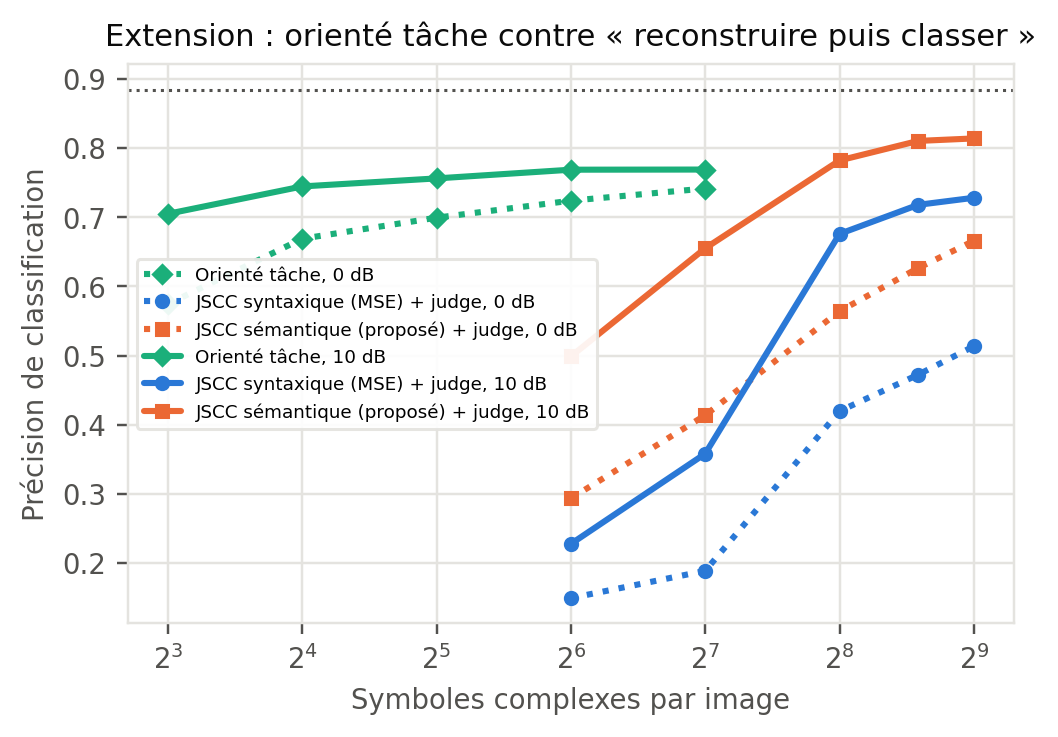
\includegraphics[width=0.88\linewidth]{task_oriented.png}
  \caption{Orienté tâche contre « reconstruire puis classer », en fonction du nombre de symboles par image.}
  \label{fig:task}
\end{figure}

\begin{keybox}[Interprétation]
L'information nécessaire à une décision parmi dix classes est très inférieure à celle qui décrit une image.
La contrepartie est l'absence de polyvalence : ce récepteur ne sait que classer, il ne peut pas afficher
l'image.
\end{keybox}

\section{Renouvellement conditionnel en vidéo}
\label{sec:cr}

Deux trames consécutives se ressemblent. L'extension envoie une image clé complète, puis uniquement les
\emph{blocs latents qui ont changé} ; le récepteur conserve les précédents pour les zones stables. La
signalisation des blocs renouvelés représente 12,7\,\% du débit et est comptée dans le rapport annoncé. Les
résultats correspondent à $\mathrm{frac} = 0{,}2$ et $c = 8$.

\begin{table}[H]
\centering
\caption{Renouvellement conditionnel contre transmission image par image, \SI{10}{\decibel}}
\label{tab:cr}
\small
\begin{tabularx}{\textwidth}{@{}lccc>{\raggedright\arraybackslash}X@{}}
\toprule
\textbf{Séquence} & \textbf{$k/n$ (CR)} & \textbf{PSNR CR} & \textbf{PSNR à $1/12$} & \textbf{Lecture} \\
\midrule
\srcfile{akiyo} (statique)           & $1/37$ & 26,40 & 26,48 & même qualité, 3 fois moins de bande \\
\srcfile{foreman} (modéré)           & $1/37$ & 25,15 & 28,06 & \SI{2.9}{\decibel} perdus \\
\srcfile{bus} (panoramique rapide)   & $1/37$ & 18,50 & 25,32 & \SI{6.8}{\decibel} perdus \\
\bottomrule
\end{tabularx}
\end{table}

\begin{figure}[H]
  \centering
  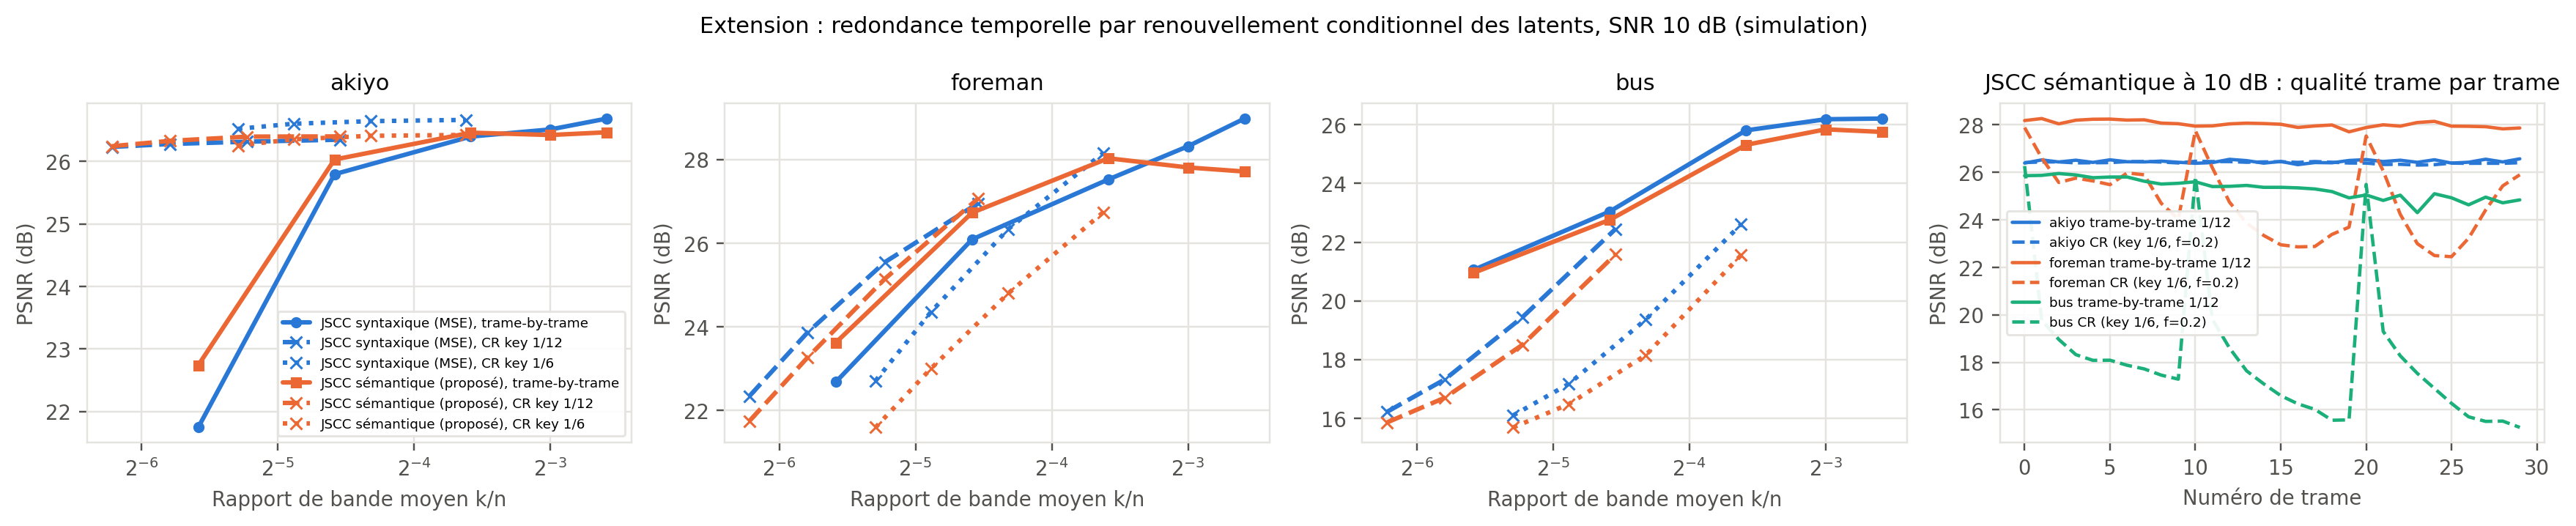
\includegraphics[width=0.76\linewidth]{video_rate.png}
  \caption{Débit effectivement utilisé au fil des trames, pour les trois régimes de mouvement.}
  \label{fig:video_rate}
\end{figure}

\begin{keybox}[Un résultat conditionnel]
La méthode exploite la redondance temporelle : elle n'apporte rien là où cette redondance n'existe pas. Le
résultat n'est pas « le renouvellement conditionnel fonctionne », mais « il fonctionne sur les scènes
statiques et doit être désactivé sur les scènes très mobiles ». Un système réel le piloterait par une mesure
de mouvement.
\end{keybox}

% ============================================================================
%  CHAPITRE 8 -- SIMULATEUR INTERACTIF
% ============================================================================
\chapter{Simulateur interactif}
\label{chap:simulateur}

Les courbes du chapitre~\ref{chap:resultats} donnent des moyennes sur des milliers d'images, mais ne montrent
pas ce qui se passe \emph{à l'intérieur} d'une transmission. Le simulateur la déroule étape par étape.

\begin{lstlisting}[language=bash, caption={Lancement}, label={lst:explore}]
python scripts/explore.py          # ouvre http://127.0.0.1:8077/
\end{lstlisting}

\section{Principe}
\label{sec:sim_principe}

Aucune étape n'est rejouée ni pré-enregistrée : chaque étape appelle le code du projet
(\srcfile{semcom.channel}, \srcfile{semcom.digital}, \srcfile{semcom.models}, \srcfile{semcom.metrics}). Ce
que la page affiche est donc ce que \srcfile{scripts/evaluate.py} mesure. Le simulateur observe la chaîne, il
ne la réimplémente pas.

\begin{table}[H]
\centering
\caption{Modules du simulateur}
\label{tab:sim_modules}
\small
\begin{tabularx}{\textwidth}{@{}p{3.3cm}>{\raggedright\arraybackslash}X@{}}
\toprule
\textbf{Module} & \textbf{Rôle} \\
\midrule
\srcfile{explorer/trace.py} & exécute une transmission et enregistre chaque étape \\
\srcfile{explorer/catalog.py} & systèmes, images et options ; chargement des modèles \\
\srcfile{explorer/encode.py} & conversion des tenseurs en objets affichables \\
\srcfile{explorer/server.py} & serveur HTTP et API JSON \\
\srcfile{explorer/static/} & carte animée, lecteur d'étapes, inspecteur, courbes \\
\bottomrule
\end{tabularx}
\end{table}

Le serveur repose sur \srcfile{http.server} et l'interface sur du HTML, CSS et JavaScript sans bibliothèque :
aucune dépendance n'est ajoutée au projet.

\section{Ce que l'on observe}
\label{sec:sim_vues}

Émetteur, canal et récepteur forment une carte sur laquelle progresse l'étape courante. Chaque étape affiche
la grandeur réellement présente à cet endroit :

\begin{itemize}
  \item le \textbf{tenseur latent} en pile 3D, canaux transmis en couleur et canaux tronqués en gris ;
  \item les \textbf{symboles I/Q} avant et après bruit : nuage continu pour le JSCC, constellation discrète
        pour la QAM ;
  \item les \textbf{bits codés}, bits faux marqués, avec le taux d'erreur avant et après Viterbi ;
  \item les \textbf{LLR} signés ; l'\textbf{image reçue} ; le \textbf{verdict des juges}.
\end{itemize}

Quatre onglets : \emph{Explorer}, \emph{Comparer} (plusieurs systèmes sur la même image, calculés en direct),
\emph{Résultats mesurés} (courbes lues dans les CSV) et \emph{Concepts}. L'état tient dans l'URL, donc une
étape précise se partage par lien.

\section{Apports}
\label{sec:sim_apport}

\paragraph{Pédagogique.} L'onglet \emph{Comparer} à \SI{2}{\decibel} montre la thèse du projet en une vue : la
chaîne séparée rend une image grise, le JSCC syntaxique une image reconnaissable mais mal classée, le JSCC
sémantique une image correctement classée.

\paragraph{Vérification.} Les grandeurs intermédiaires rendent observables des comportements que les moyennes
masquent : le budget binaire insuffisant pour un seul canal latent aux MCS robustes
(section~\ref{sec:codage_source}), ou le fait que très en dessous du seuil, Viterbi peut produire un taux
d'erreur \emph{supérieur} au taux brut en s'engageant sur un mauvais chemin du treillis. Deux conséquences
correctes de la théorie, invisibles sur une courbe de PSNR.

% ============================================================================
%  CONCLUSION GÉNÉRALE ET PERSPECTIVES
% ============================================================================
\chapter*{Conclusion générale et perspectives}
\addcontentsline{toc}{chapter}{Conclusion générale et perspectives}
\markboth{Conclusion générale et perspectives}{Conclusion générale et perspectives}

Trois manières de franchir un canal bruité simulé ont été comparées sous un budget radio identique : la
chaîne séparée simulée bit à bit, un codage conjoint appris sur une perte pixel, et le même réseau entraîné
avec une perte sémantique. Le dispositif a été construit pour que la comparaison soit recevable —
architecture identique entre les deux systèmes appris, puissance normalisée, canal et tirages communs, chaîne
numérique non approchée, juges absents de toute fonction de perte.

\paragraph{Résultats.} Ajouter à la perte un terme de caractéristiques et un terme de tâche, et rien d'autre,
échange environ \SI{0.5}{\decibel} de PSNR contre 10 à 14~points de précision chez un juge indépendant, en
AWGN comme en Rayleigh. En supprimant les bits, le codage conjoint supprime l'effet falaise : à
\SI{0}{\decibel}, là où la chaîne séparée réelle tombe au niveau du hasard, les systèmes appris restent
exploitables. Enfin, un modèle entraîné à SNR fixe est inutilisable ailleurs : l'entraînement sur une plage
est la condition d'un système déployable.

\paragraph{Limites.} Le canal est simulé et la CSI supposée parfaite sous Rayleigh. Les modèles n'ont vu que
des images $32\times32$ : sur Kodak et en vidéo, la borne idéale de la chaîne séparée reste devant en PSNR,
ce qui est un résultat de transfert et non une défaite de principe. La borne de capacité, enfin, n'est pas un
système constructible.

\paragraph{Extensions.} Quand la tâche du récepteur est connue, la transmission orientée tâche atteint une
précision comparable avec 32 fois moins de bande. Quand le contenu est temporellement redondant, le
renouvellement conditionnel divise la bande par trois sur une scène statique — et doit être désactivé
ailleurs.

\paragraph{Perspectives.} À court terme, l'\textbf{entraînement sur images naturelles}, seul moyen de
trancher la comparaison avec JPEG sur Kodak, et le \textbf{pilotage automatique du renouvellement
conditionnel} par une mesure de mouvement. À moyen terme : une \textbf{estimation imparfaite du canal},
l'étude du gain sémantique pour \textbf{d'autres tâches} que la classification, et une \textbf{quantification
des symboles émis}, nécessaire pour rencontrer un émetteur radio réel. À plus long terme, la validation sur
une radio logicielle reste l'étape qui manque pour passer d'une démonstration en simulation à un résultat de
transmission.


% --------------------------------------------------------------- fin de document
\phantomsection
\addcontentsline{toc}{chapter}{Bibliographie}
\bibliographystyle{ieeetr}
{\small\setstretch{1.0}\bibliography{references}}

\appendix
% ============================================================================
%  ANNEXES
% ============================================================================
\chapter{Reproduction des résultats}
\label{app:repro}

L'ensemble de la campagne est relançable depuis la racine du projet. Les modèles déjà entraînés sont ignorés,
de sorte que la commande peut être relancée après une interruption.

\begin{lstlisting}[language=bash, caption={Installation et campagne complète}, label={lst:repro}]
python -m venv .venv
.venv\Scripts\activate              # Linux/macOS : source .venv/bin/activate
pip install -r requirements.txt
python scripts/download_data.py     # CIFAR-10, Kodak, 3 clips Xiph, poids ResNet-18 (~250 Mo)

python scripts/run_all.py --workers 4 --threads 4    # entraine les 9 modeles
python scripts/evaluate.py all --workers 6           # -> results/eval/*.csv
python scripts/make_figures.py                       # tableaux et figures
python scripts/demo.py                               # comparaison visuelle
python scripts/explore.py                            # simulateur interactif
\end{lstlisting}

Sur un processeur à 16 fils d'exécution, la campagne d'entraînement demande environ \SI{2.5}{\hour} et
l'évaluation environ \SI{30}{\minute}. Les données ne sont pas versionnées — \SI{391}{\mega\byte}, dont des
fichiers dépassant la limite de \SI{100}{\mega\byte} par fichier des dépôts Git ; le script de téléchargement
les régénère.

\chapter{Fichiers de résultats produits}
\label{app:fichiers}

\begin{table}[H]
\centering
\caption{Fichiers de résultats et contenu}
\label{tab:fichiers}
\small
\begin{tabularx}{\textwidth}{@{}p{5.1cm}>{\raggedright\arraybackslash}X@{}}
\toprule
\textbf{Fichier} & \textbf{Contenu} \\
\midrule
\srcfile{results/eval/cifar_analog.csv} & JSCC syntaxique et sémantique, modèles à SNR fixe, orienté tâche, sur CIFAR-10 \\
\srcfile{results/eval/cifar_digital.csv} & chaîne séparée simulée bit à bit, un point par MCS et par SNR \\
\srcfile{results/eval/cifar_capacity.csv} & borne de capacité de la chaîne séparée sur CIFAR-10 \\
\srcfile{results/eval/kodak_jscc.csv} & systèmes appris sur les 24 images Kodak \\
\srcfile{results/eval/kodak_sep.csv} & chaîne séparée JPEG sur Kodak, et sa borne de capacité \\
\srcfile{results/eval/video_jscc.csv} & systèmes appris et renouvellement conditionnel sur les 3 clips \\
\srcfile{results/eval/video_sep.csv} & chaîne séparée JPEG sur les 3 clips \\
\srcfile{results/eval/video_frames.csv} & qualité trame par trame \\
\srcfile{results/tables/summary.md} & tableau de synthèse au point $k/n = 1/12$ \\
\srcfile{results/tables/models.csv} & paramètres, époques et durées d'entraînement des neuf modèles \\
\bottomrule
\end{tabularx}
\end{table}

\chapter{Paramètres de simulation}
\label{app:params}

\begin{table}[H]
\centering
\caption{Valeurs numériques employées dans toute la campagne}
\label{tab:params}
\small
\begin{tabularx}{\textwidth}{@{}p{6.2cm}>{\raggedright\arraybackslash}X@{}}
\toprule
\textbf{Paramètre} & \textbf{Valeur} \\
\midrule
Canaux latents (total) & 16, au stride 4 \\
Canaux transmis $c$ & 2, 4, 8, 12, 16 soit $k/n$ de $1/48$ à $1/6$ \\
Point de fonctionnement principal & $k/n = 1/12$ ($c = 8$) \\
Plage de SNR & 0 à \SI{20}{\decibel} ; pas de \SI{1}{\decibel} sur CIFAR-10, \SI{2}{\decibel} ailleurs \\
Puissance moyenne par symbole & 1 \\
Poids de la perte sémantique & $\lambda_f = 0{,}01$ ; $\lambda_t = 0{,}003$ \\
Optimiseur & Adam, pas $10^{-3}$, lots de 128 \\
Code convolutif & $K = 7$, polynômes $(133,171)_8$ \\
Rendements & 1/2, 2/3, 3/4 (poinçonnage 802.11a) \\
Modulations & QPSK, 16-QAM, 64-QAM, codage de Gray \\
Taille de paquet & \num{1024} bits utiles au maximum, 6 bits de queue \\
Images d'évaluation & \num{5000} (CIFAR-10), 24 (Kodak), $3\times30$ trames (vidéo) \\
\bottomrule
\end{tabularx}
\end{table}


\end{document}
